%================================================================== Logo On/Off
\LogoOff

%==================================================================FRONT PAGE AND TOC
% For article only
\mode<presentation:0>{\thispagestyle{empty}\maketitle}

% For presentation only
\mode<presentation| article:0| handout:0>{
    \begin{frame}<article:0>[label=portada]
    \titlepage
    \end{frame}%Fin del frame
}

% For handout only
\mode<handout>{
  \begin{frame}[label=portada]
    \maketitle
  \end{frame}
}

%% TABLE OF CONTENTS
\begin{frame}[label=toc]
    \mode<article:0>{\frametitle{Contents}}
    \mode<presentation>{\small}
    \tableofcontents%[hidesubsections]
\end{frame}

%%%==================================================================S INTRODUCTION
\section[ALS]{\textquestiondown Qué es el LiDAR aéreo?}
%%%==================================================================Sb
%\subsection{Principios}
%%%==================================================================F 
%\begin{frame}
%    \frametitle{Principios del LiDAR aéreo}
%    \begin{enumerate}
%        \item El LiDAR aéreo (Airborne Laser Scanner, \alert<1>{ALS}) es la combinación de:
%	\uncover<1->{
%	\begin{itemize}
%	 \item \alert<1,2>{Escaner Laser}
%	 \item \alert<1,3>{GPS}, que nos da la posición del sensor.
%	 \item \alert<1,3>{IMU}, que nos da nuestra orientación del avión.
%	\end{itemize}
%	}
%	\uncover<2->{
%	\item La posición con respecto al sensor de un punto en tierra se determina por:
%	\begin{itemize}
%	 \item El \alert<2>{tiempo} que tarda cada impulso desde que es emitido hasta que es recibido.
%	 \item El \alert<2>{ángulo} medido desde el nadir en el cual ha sido emitido el rayo.
%	\end{itemize}
%	}
%	\uncover<3>{\item  La posición relativa combinada con la posición global (\alert<3>{GPS}) y la orientación (\alert<3>{IMU}) nos permiten calcular las coordenadas (X,Y,Z) en el punto medido en tierra en un sistema de posicionamiento global (WGS84)}
%    \end{enumerate}
%\end{frame}
%%%==================================================================Sb
%\subsection{Características}
%%%==================================================================F
%\begin{frame}[label=lidar_charact]
%    \frametitle{Características del ALS}
%    \begin{enumerate}[<+->]
%    	\item \alert<1>{Alta precisión} tanto en la componente planimétrica como en la altrimétrica
%    	\item \alert<2>{Alta resolución} debido a la frecuencia de medición.
%    	\item \alert<3>{Monoscópica} y casi \alert{nadiral} $\Rightarrow$ permite observar el terreno incluso en zonas de gran vegetación
%    \end{enumerate}
%\end{frame}
%%==================================================================Sb
\subsection{Primer y último impulso}
%%==================================================================F 
\mode<beamer>{
  \pgfdeclareimage[height=40mm]{roof}{images/roof}
  \pgfdeclareimage[height=40mm]{tree}{images/tree}
}
\mode<beamer:0>{
  \pgfdeclareimage[height=40mm]{roofg}{images/roof_grey}
  \pgfdeclareimage[height=40mm]{treeg}{images/tree_grey}
}
\begin{frame}[label=firstlast1]
    \frametitle{Primer y último impulso}
    \begin{enumerate}[<+->]
        \item Debido a la divergencia del láser, pueden recibirse \alert<1>{más de un eco} para el mismo rayo.
	\item Los sensores actuales son capaces de medir al menos dos retornos: \alert<2>{primero} y \alert<2>{último}
	\item Normalmente se producen por: \alert<3->{bordes} de edificios \uncover<4->{o \alert<4>{vegetación}}
    \end{enumerate}
    \begin{center}
   	\begin{tikzpicture}
	\mode<beamer>{
    	  \uncover<3->{\pgftext[bottom,left,at={\pgfpointxy{-2}{0}}]{\pgfuseimage{roof}}}
    	  \uncover<4>{\pgftext[bottom,left,at={\pgfpointxy{2}{0}}]{\pgfuseimage{tree}}}
	}
	\mode<beamer:0>{
    	  \pgftext[bottom,left,at={\pgfpointxy{-2}{0}}]{\pgfuseimage{roofg}}
    	  \pgftext[bottom,left,at={\pgfpointxy{2}{0}}]{\pgfuseimage{treeg}}
	}
	\end{tikzpicture}
    \end{center}
\end{frame}
%%==================================================================F 
\begin{frame}
    \frametitle{\textquestiondown Para qué sirve?}
    \begin{enumerate}[<+->]
     \item Una diferencia considerable entre el primer y último impulso puede ser una pista para detectar vegetación y otros objetos: edificios, puentes, tendidos eléctricos...
     \item Los últimos impulsos tienen más probabilidad de ser terreno.
     \item Mediante una simple interpolación:
     	\begin{itemize}
     	   \item Primer impulso: creación de Modelo Digital de Superficie (\alert<4>{DSM})
     	   \item \'Ultimo impulso: ``creación'' de Modelo Digital del Terreno (\alert<5>{DTM})
     	\end{itemize}
     \item Hay pocas posibilidades de, sin hacer ningún análisis, distinguir entre un punto \alert<6>{objeto} y uno \alert<6>{terreno}.
    \end{enumerate}
\end{frame}
%%==================================================================S
\section[Filtros]{Filtros ALS}
%%==================================================================Sc
\subsection{Definición}
%%==================================================================F
\begin{frame}[label=filter_def]
    \frametitle{Filtros ALS}
    \onslide<1->\begin{beamerboxesrounded}[shadow=true]{Definición: \emph{Nube de puntos LiDAR}}
     Es un conjunto de puntos tridimensionales con un atributo asociado: $V = \left\lbrace v=\left(x,a\right) | x \in \mathbb{R}^3, a \in \mathbb{N} \right\rbrace$
    \end{beamerboxesrounded}

    \onslide<2->{Clasificación la nube de puntos como:
    \begin{itemize}
 	\item 1, si el punto pertenece a un \alert<2>{objeto}
 	\item<3-> 0, si el punto pertenece al \alert<3>{terreno}
    \end{itemize}}

    \onslide<4>\begin{beamerboxesrounded}[shadow=true]{Definición: \emph{Filtrar}}
     Consiste en \alert<4>{eliminar} los puntos de $V$ con atributo igual 1 (objeto) y dejar los clasificados como 0 (terreno).
    \end{beamerboxesrounded}
\end{frame}
%%==================================================================Sb
\subsection{Tipos de filtros/clasificaciones}
%%==================================================================F
\begin{frame}
    \frametitle{Tipos de clasificaciones}
    \begin{itemize}
        \item Morfológicos
        \item Densificación progresiva
        \item Segmentación y \emph{clustering}
        \item Basado en superficies
        \item Estudio de pendientes (splines)
    \end{itemize}
\end{frame}
%%==================================================================Sb
\subsection{Comparación de filtros}
%%==================================================================F
\begin{frame}
  \frametitle{Comparación de filtros}
    \begin{itemize}
      \item Estudio del rendimiento de los 8 filtros distintos 
      \item Auspiciado por el \emph{International Society of Photogrammetry and
        Remote Sensing} (\alert{ISPRS})
      \item Estudio cualitativo y cuantitativo
    \end{itemize}
\end{frame}
%%==================================================================F
\begin{frame}
  \frametitle{Resultados}
  \begin{enumerate}
    \item Todos los filtros funcionan correctamente con escenarios poco exigentes
      \begin{itemize}
        \item Poca o nula pendiente, y extensas zonas de terreno
        \item Pequeños edificios
        \item Vegetación dispersa
      \end{itemize}
    \item Mayores problemas en zonas con:
      \begin{itemize}
        \item Edificios voluminosos con escasa extensión de terreno
        \item Parches de terreno a diferentes alturas o con alturas variables
      \end{itemize}
    \item<2-> Mejores prestaciones: \alert<2>{densificación progresiva} y los basados
      en la \alert<2>{determinación de superficies}
    \item<3-> Los más desarrollados: \alert<3>{segmentación y clustering}
    \item<4-> \alert<4>{Combinación} de varios algoritmos e \emph{inputs} distintos
  \end{enumerate}
\end{frame}
%%==================================================================F
\begin{frame}
  \frametitle{Automatización Vs Manual}
  \begin{enumerate}
    \item Comparados con la fotogrametría, los filtros son procesos \alert{automáticos}
    \item Todavía no se ha encontrado un filtro completamente automático y
      \alert{universal}
    \item \alert{Necesaria} una revisión y edición manual (cercados,
      umbrales\ldots)
      \begin{itemize}
        \item Zonas urbanas 
        \item \alert{Innecesaria en zonas rurales}
        \item Puentes y pasos elevados
        \item Algoritmos basados en relaciones geométricas de puntos vecinos
        \item El terreno no puede ser identificado por escasez de puntos
        %\item El trabajo depende de las características de la superficie
      \end{itemize}
    \item Fuentes de datos adicionales pueden disminuir la revisión
      \begin{itemize}
        \item Delimitación de edificios
        \item Contexto de terreno local
        \item Información radiométrica: \alert{externa} o la \alert{devuelta por
          el láser}
      \end{itemize}
  \end{enumerate}
\end{frame}
%%==================================================================F
\begin{frame}
  \frametitle{Densidad puntual}
  \begin{itemize}
    \item La influencia de la densidad depende fuertemente de la topografía
    \item Se necesita una densidad mínima para asegurar cierta penetración en
      zonas vegetales
    \item En zonas complejas es además importante para asegurar la
      representación de calidad de los detalles del escenario
    \item Incluso con alta densidad, los filtros presentan problemas de
      clasificación
    \item Según disminuye la densidad los resultados empobrece rápidamente
  \end{itemize}
\end{frame}
%%==================================================================Sc
\section[DTM]{Generación de Modelos Digitales del Terreno}
%%==================================================================F
\begin{frame}
  \frametitle{Modelos Digitales del Terreno (DTM)}
  \begin{beamerboxesrounded}[shadow=true]{Definición}
    Teóricamente sería una representación continua, $f$, del terreno en un
    cierto área local. Dadas las coordenadas planimétricas de un punto,
    $\mathbf{p}=(x,y)$, y su valor altimétrico asociado, $z$, la representación
    \alert<1>{2.5D} del terreno, sería: $z=f(x,y)$
  \end{beamerboxesrounded}
  \begin{itemize}
    \item<2-> \alert<2>{2.5D $\ne$ 3D}
      \begin{itemize}
        \item<3-> $z_1 = \mathbf{p}(x,y)$; $z_2 = \mathbf{p}(x,y)$ \alert<3>{¡!}
        \item<4-> Puentes y pasos elevados $\Rightarrow$ \alert<4>{No se consideran}
      \end{itemize}
  \end{itemize}
\end{frame}
%%==================================================================F
\begin{frame}
  \frametitle{Tipos de Modelos digitales}
  \begin{minipage}{.4\textwidth}
  \begin{enumerate}[<+->]
    \item Realidad
    \item Modelo Digital de Superficie (DSM)
    \item Modelo de Edificios (DBM)
    \item Modelo Digital del Terreno (DTM)
  \end{enumerate}
  \end{minipage}
  \begin{minipage}{.55\textwidth}
    \uncover<1->{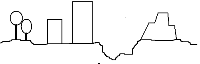
\includegraphics[height=0.20\textheight]{images/realidad}}
    \uncover<2->{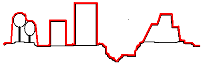
\includegraphics[height=0.20\textheight]{images/dsm}}
    \uncover<3->{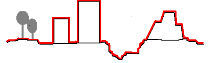
\includegraphics[height=0.20\textheight]{images/dbm}}
    \uncover<4->{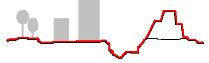
\includegraphics[height=0.20\textheight]{images/dtm}}
  \end{minipage}
\end{frame}
%%==================================================================F
\begin{frame}
  \frametitle{DTM Vs. DSM}
  \begin{enumerate}
    \item \alert{DTM}
    \begin{itemize}
      \item Se busca un suavizado de la superficie
      \item Se utilizan los últimos ecos para filtrar
    \end{itemize}
    \item \alert{DSM}
    \begin{itemize}
      \item Se busca resaltar los detalles
      \item Se utilizan los primeros impulsos
      \item Errores en observaciones groseras $\Rightarrow$ \alert{Limpiar}
      \item Objetos temporales (coches, gruas\ldots) $\Rightarrow$ \alert{Limpiar}
    \end{itemize}
  \end{enumerate}
\end{frame}
%%==================================================================F
\begin{frame}
  \frametitle{nDSM}
    \begin{itemize}
      \item \alert{nDSM = DSM - DSM}
    \end{itemize}
    \begin{center}
      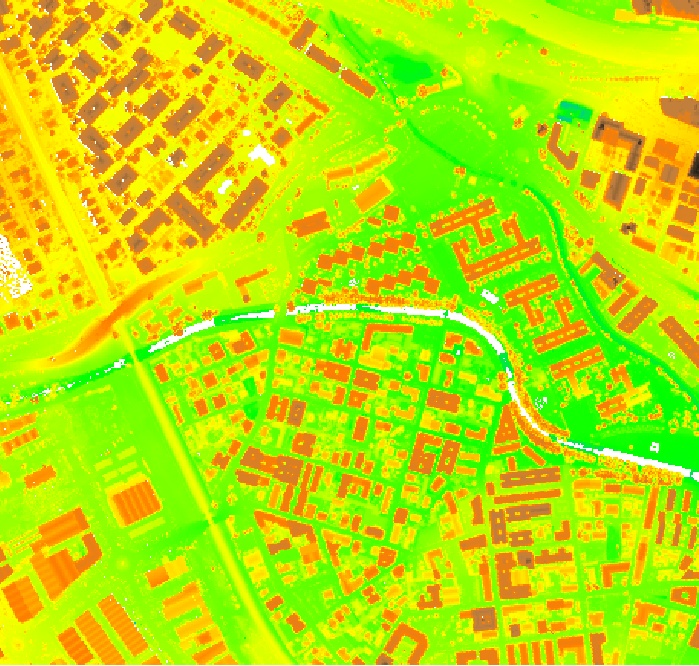
\includegraphics[width=0.30\textwidth]{images/n_dsm}~--~
      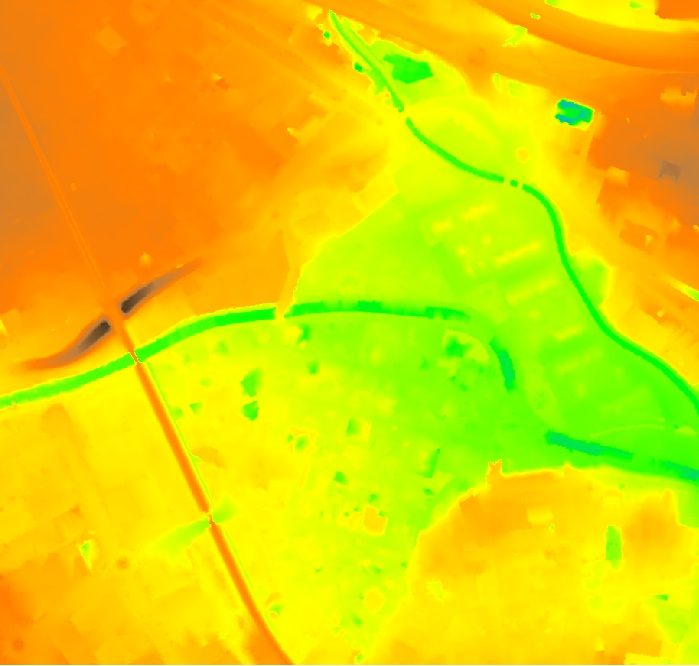
\includegraphics[width=0.30\textwidth]{images/n_dtm}~$\Rightarrow$~
      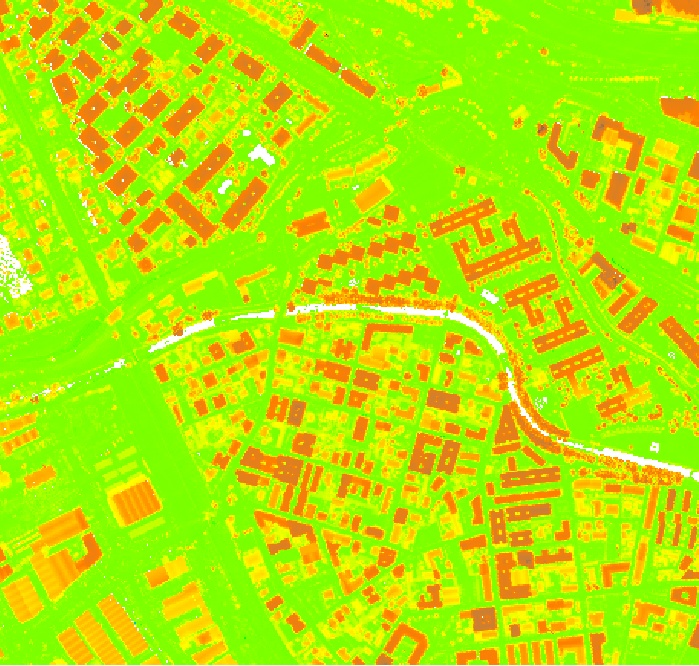
\includegraphics[width=0.30\textwidth]{images/n_ndsm}~
    \end{center}
\end{frame}
%%==================================================================Sb
\subsection[Ráster]{Estructuras regulares}
%%==================================================================F
\begin{frame}
  \frametitle{Continuo Vs. Discreto}
  \begin{enumerate}
    \item Interesa almacenar la representación del DTM una vez conocida
    \item Opción: definición de la funcion $z = f(x,y)$ + el área
      \begin{itemize}
        \item[\tickYes] Realmente continuo
        \item[\tickNo] No siempre es conocida
        \item[\tickNo] No es algo estándar
      \end{itemize}
    \item Discretización en un intervalos regulares
      \begin{itemize}
        \item[\tickNo] No es continuo
        \item[\tickYes] Fácilmente almacenable
        \item[\tickYes] Existen multitud de formatos ``estándar''
      \end{itemize}
  \end{enumerate}
\end{frame}
%%==================================================================F
\begin{frame}
  \frametitle{Raster Vs. Mallado}
  \begin{enumerate}
    \item<1-> \alert{Ráster} 
      \begin{itemize}
        \item Cada celda representa la altura de todo el área que cubre la celda
      \end{itemize}
    \item<2-> Malla
      \begin{itemize}
        \item Representa la información de altura en puntos regularmente ordenados
        \item Cada altura es la evaluación de $f$ en cada punto $(x,y)$ de la
          malla
        \item Interpolación, aproximación (inverso de la distancia pesada),
          mínimos cuadrados móviles, kriging, etc,\ldots
      \end{itemize}
        \item<3-> Son uno el dual del otro
    \item<4-> Se suelen confundir
  \end{enumerate}
\end{frame}
%%==================================================================F
\begin{frame}
  \frametitle{Raster Vs. Mallado}
  \begin{itemize}
    \item Ráster 
  \end{itemize}
  \begin{center}
        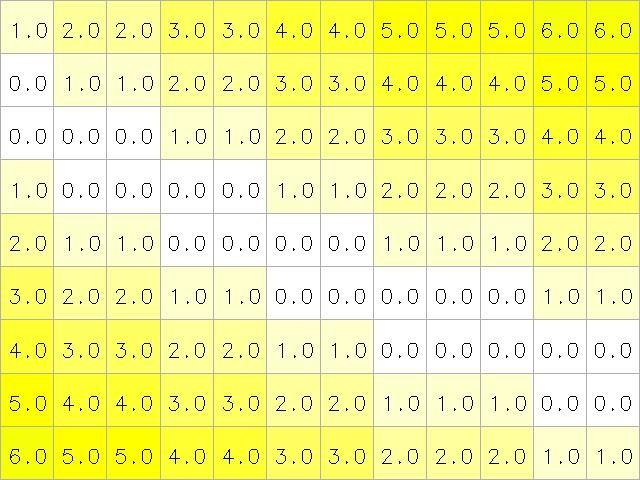
\includegraphics[height=0.60\textheight]{images/raster}
  \end{center}
\end{frame}
%%==================================================================F
\begin{frame}
  \frametitle{Raster Vs. Mallado}
  \begin{itemize}
    \item Malla 
  \end{itemize}
  \begin{center}
        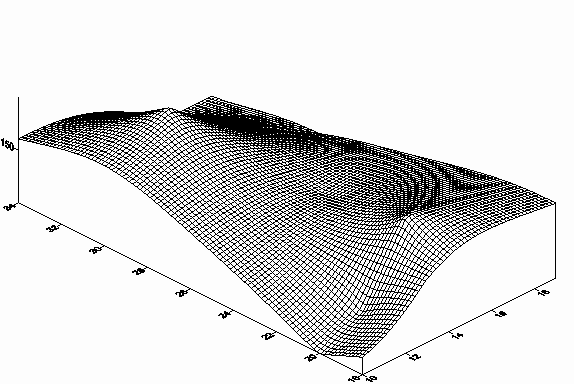
\includegraphics[height=0.60\textheight]{images/mallado}
  \end{center}
\end{frame}
%%==================================================================F
\begin{frame}
  \frametitle{Raster Vs. Mallado}
  \begin{itemize}
    \item Malla híbrida 
  \end{itemize}
  \begin{center}
        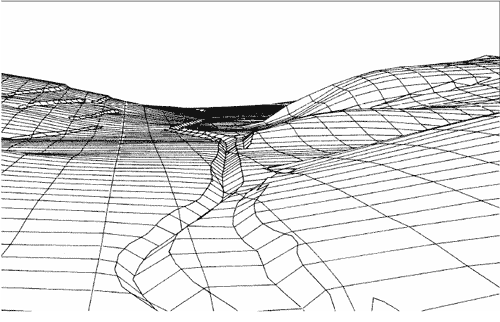
\includegraphics[height=0.60\textheight]{images/malla_breaklines}
  \end{center}
\end{frame}
%%==================================================================Sb
\subsection{TIN}
%%==================================================================F
\begin{frame}
  \frametitle{TIN}
  \begin{enumerate}
    \item \alert{TIN}: \emph{Triangulated irregular network}
    \item Los puntos topológicamente vecinos deben guardar unas reglas
      geométricas: \alert{Triangulación de Delaunay}
    \item Permiten también modelos híbridos con líneas de ruptura
    \item Formatos estándares
  \end{enumerate}
\end{frame}
%%==================================================================F
\begin{frame}
  \frametitle{TIN}
  \begin{itemize}
    \item Triangulación
  \end{itemize}
  \begin{center}
        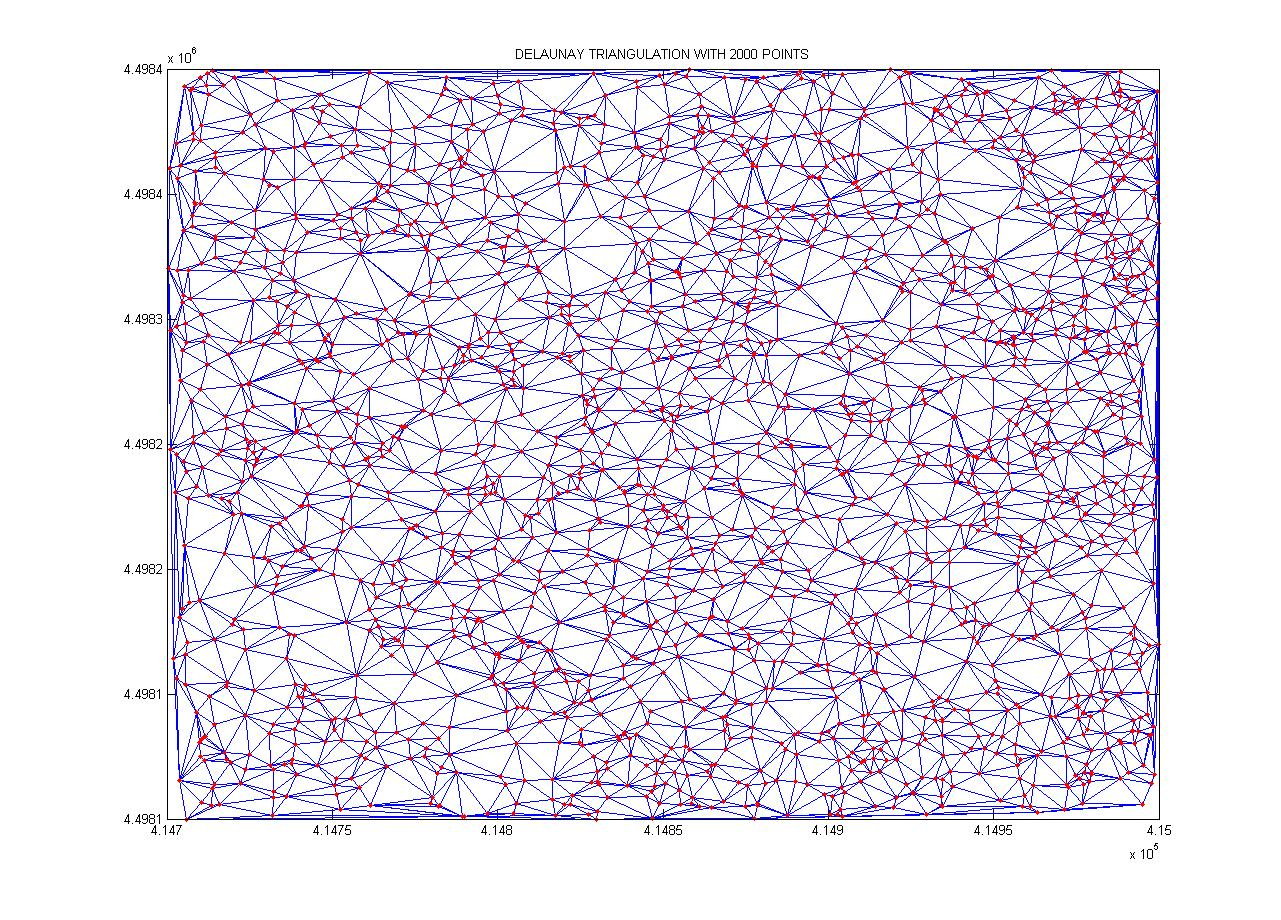
\includegraphics[height=0.60\textheight]{images/triangulacion}
  \end{center}
\end{frame}
%%==================================================================F
\begin{frame}
  \frametitle{TIN}
  \begin{itemize}
    \item \alert{NO} este TIN :-)
  \end{itemize}
  \begin{center}
        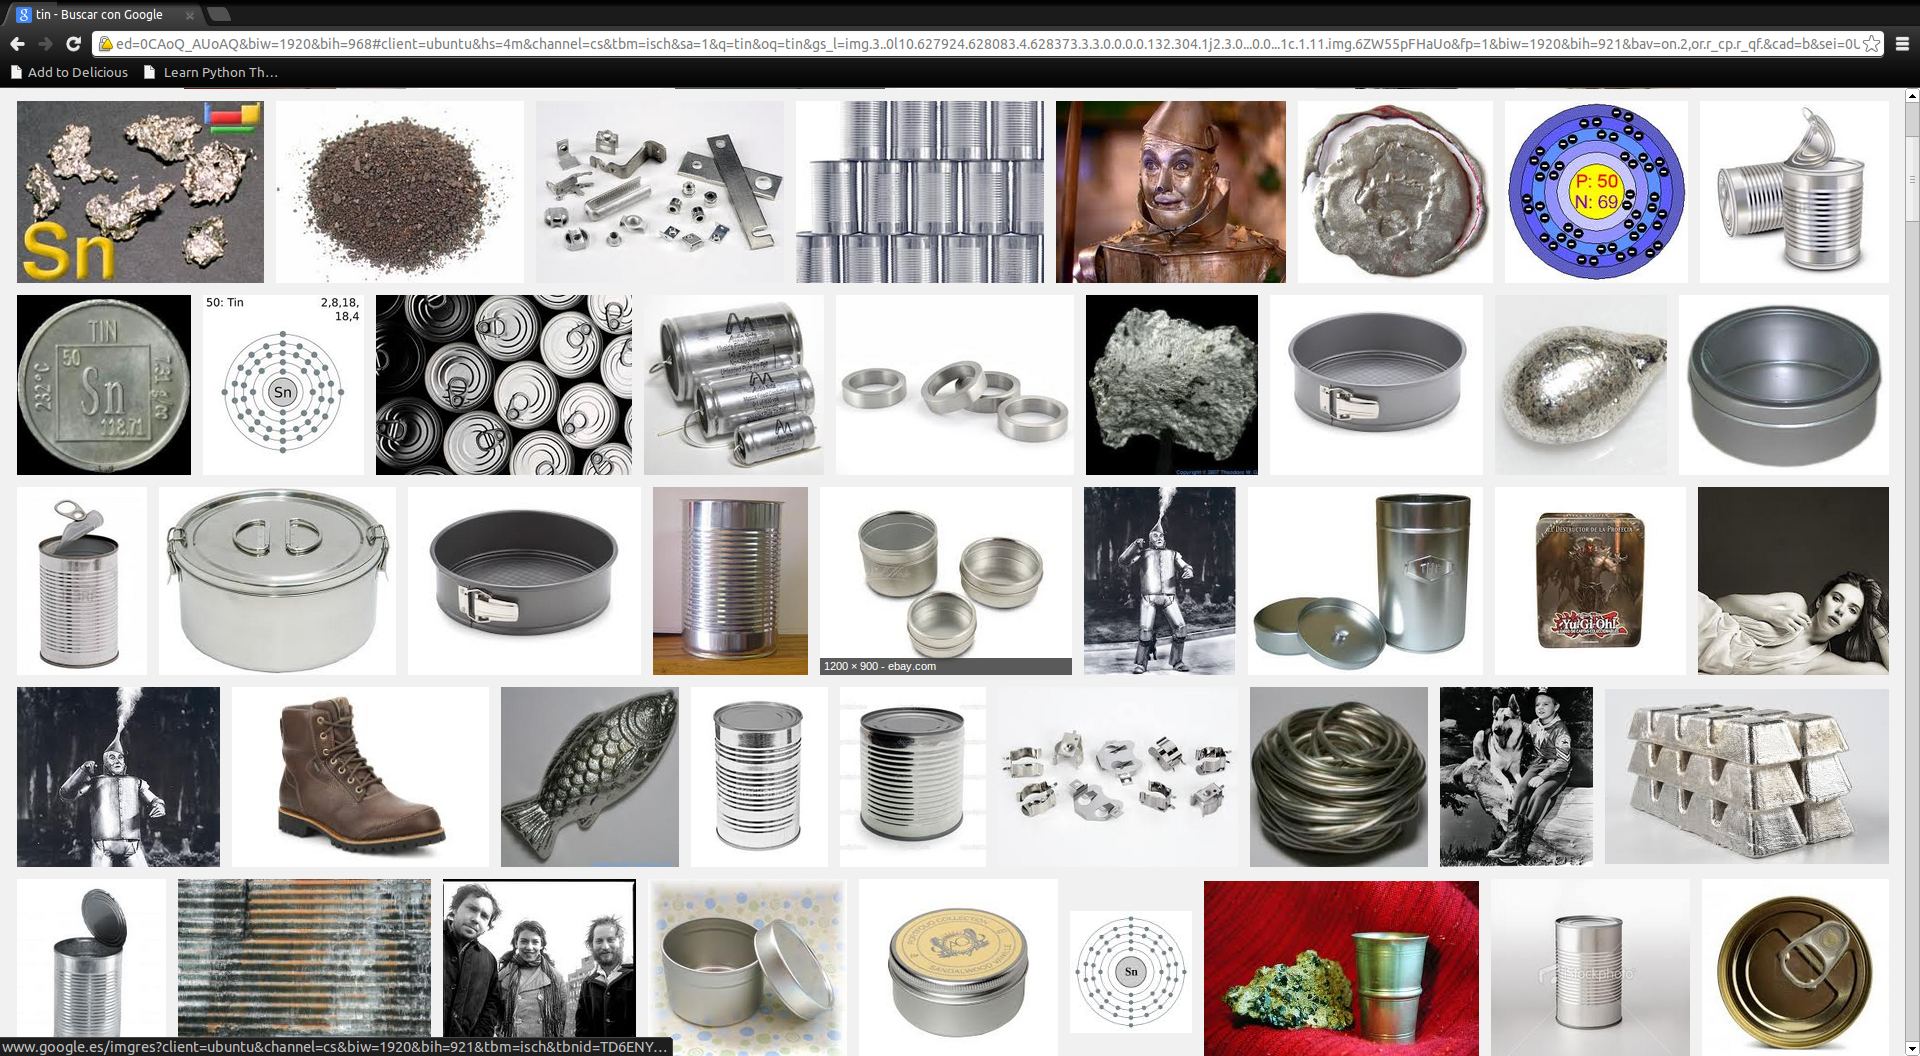
\includegraphics[height=0.60\textheight]{images/estano}
  \end{center}
\end{frame}
%%==================================================================F
\begin{frame}
  \frametitle{TIN}
  \begin{itemize}
    \item TIN
  \end{itemize}
  \begin{center}
        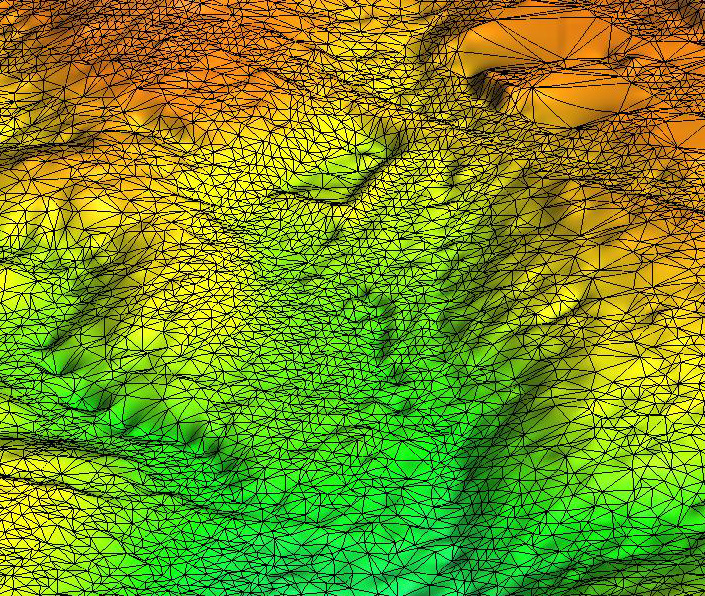
\includegraphics[height=0.60\textheight]{images/tin_dem}
  \end{center}
\end{frame}
%%==================================================================F
\begin{frame}
  \frametitle{Triangulación de Delaunay}
  \begin{beamerboxesrounded}[shadow=true]{Definición: \emph{Triangulación de
    Delaunay}}
    Sea $P$ un conjunto de puntos en el \alert{plano}, se dice que $T$ es una
    \alert{\emph{Triangulación de Delaunay}} $\Leftrightarrow$ cualquier círculo que
    circunscriba cualquier triángulo de $T$ no encierra ningún otro punto de $P$
    \end{beamerboxesrounded}
  \begin{enumerate}
    \item La mejor aproximación posible genera triángulos regulares
    \item En cualquier caso: maximiza el menor ángulo de cada triángulo
  \begin{center}
        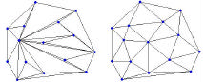
\includegraphics[height=0.15\textwidth]{images/triang_regular}
  \end{center}
  \end{enumerate}
\end{frame}
%%==================================================================F
\begin{frame}
  \frametitle{Triangulación de Delaunay}
  \begin{beamerboxesrounded}[shadow=true]{Propiedad 1}
    Sea $P$ un conjunto de puntos en el plano, entonces tres puntos $p_i, p_j$ y
    $p_k$ son vértices del mismo triángulo de la triangulación de Delaunay de $P
    \Leftrightarrow$ la circunferencia que pasa por los tres puntos no encierra
    ningún punto de $P$
  \end{beamerboxesrounded}
  \begin{center}
  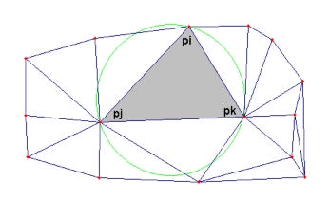
\includegraphics[height=0.20\textwidth]{images/propiedad1}
  \end{center}
\end{frame}
%%==================================================================F
\begin{frame}
  \frametitle{Triangulación de Delaunay}
  \begin{beamerboxesrounded}[shadow=true]{Propiedad 2}
    Sea $P$ un conjunto de puntos en el plano, entonces, dos puntos, $p_i$ y
    $p_j$ forman un segmento de la triangulación de Delaunay de $P
    \Leftrightarrow$ existe una circunferencia que contiene a ambos pero no
    encierra ningún punto de $P$
  \end{beamerboxesrounded}
  \begin{center}
  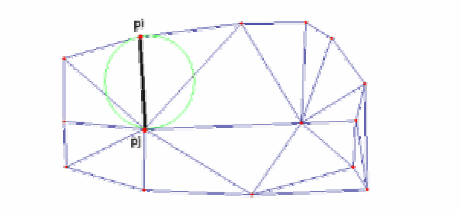
\includegraphics[height=0.20\textwidth]{images/propiedad2}
  \end{center}
\end{frame}
%%==================================================================Sb
\subsection[Calidad]{Calidad de los DTM}
%%==================================================================F
\begin{frame}
  \frametitle{Calidad de los DTM}
  \begin{enumerate}
    \item<1-> \alert<1>{Calidad de los datos}
      \begin{itemize}
        \item Describe la calidad de los datos de entrada
      \end{itemize}
    \item<2-> \alert<2>{Calidad del modelo}
      \begin{itemize}
        \item Describe la calidad del modelo final generado
      \end{itemize}
  \end{enumerate}
\end{frame}
%%==================================================================F
\begin{frame}
  \frametitle{Calidad de los datos}
  \begin{enumerate}
    \item Capa de densidad de puntos
      \begin{itemize}
        \item Permite identificar zonas con escasez de datos
        \item Ofrece información sobre las posibles interpolaciones y
          extrapolaciones
      \end{itemize}
    \item Capa de distancia entre puntos
      \begin{itemize}
        \item Parecida al mapa de densidad
        \item Permite conocer zona con pocos puntos
        \item Da información sobre la distancia del vecino más próximo
      \end{itemize}
    \item Fuentes de datos
      \begin{itemize}
        \item Da información sobre la presencia de distintos tipos de inputs:
          ALS, TLS, fotogrametría, etc\ldots
      \end{itemize}
    \item Mapa de precisión de las fuentes de datos
      \begin{itemize}
        \item Da información sobre la mejor o peor precisión de los datos
      \end{itemize}
  \end{enumerate}
\end{frame}
%%==================================================================F
\begin{frame}
  \frametitle{Calidad de los datos}
  \only<1,2>{Pasadas
    \begin{center}
      \only<1>{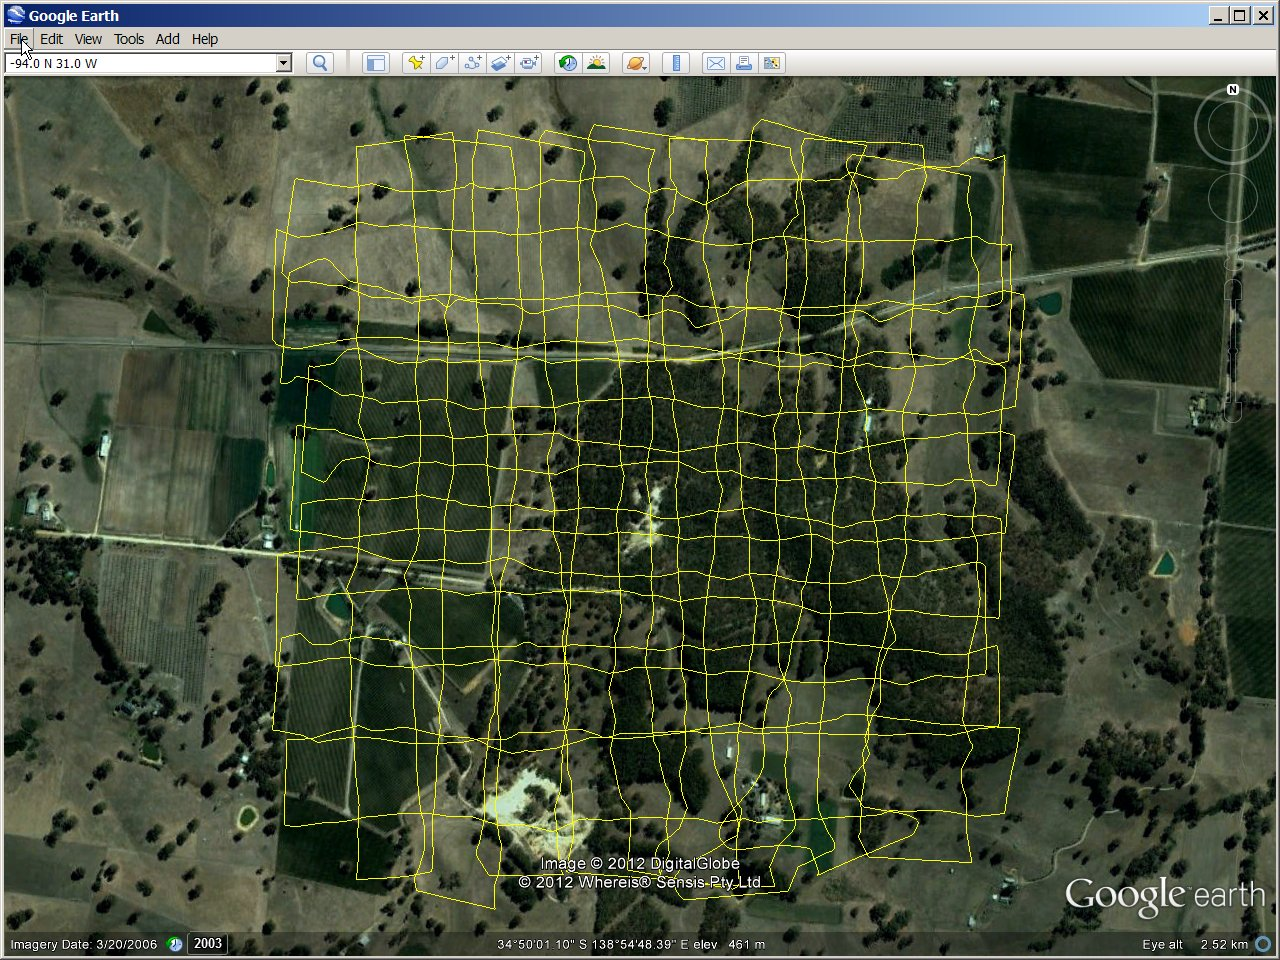
\includegraphics[width=0.55\textwidth]{images/pasadas}}
      \only<2>{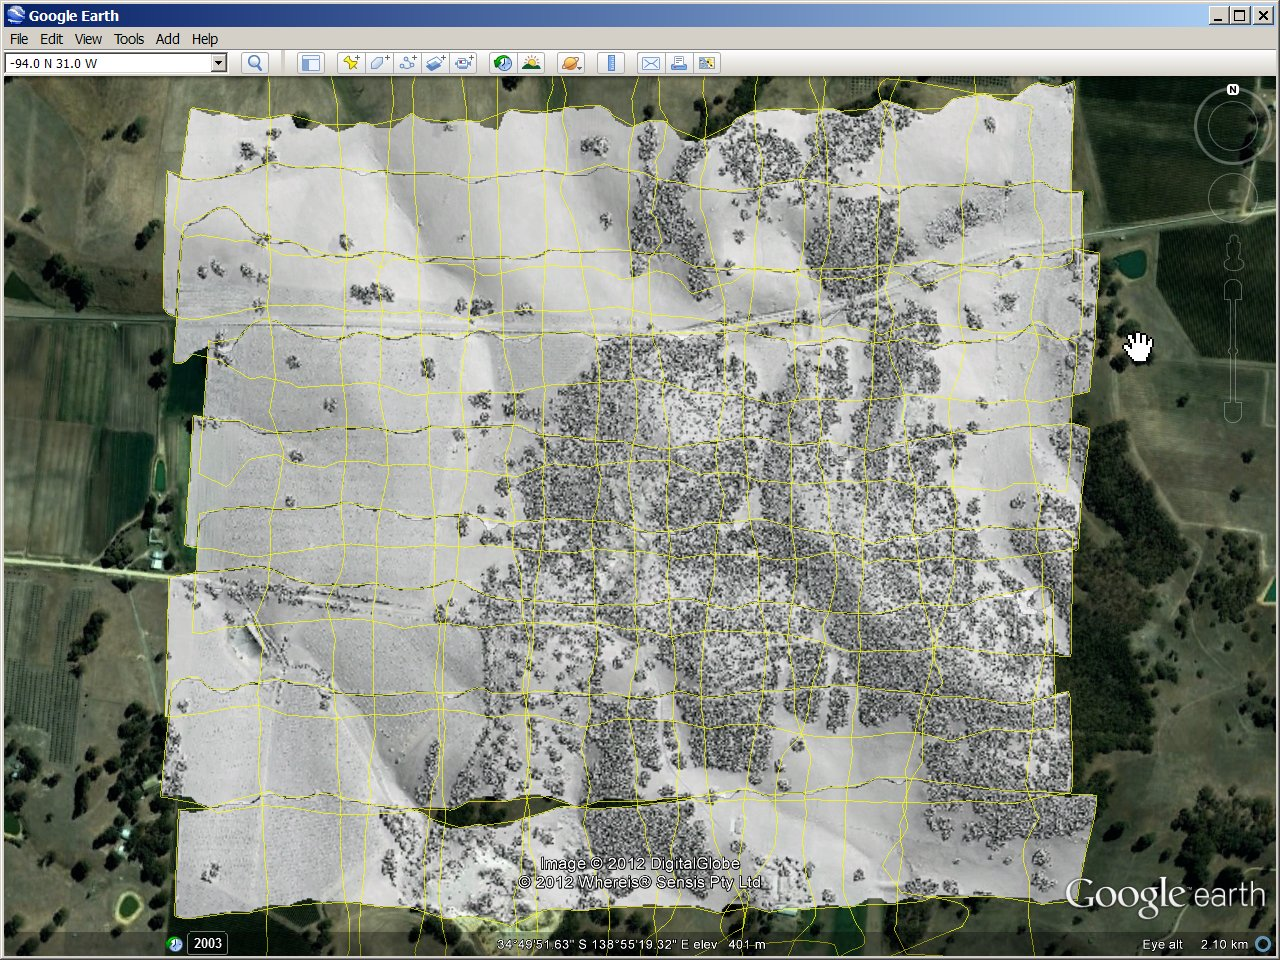
\includegraphics[width=0.55\textwidth]{images/pasadas_shademap}}
    \end{center}
  }
  \only<3>{Mapa de densidades
    \begin{center}
      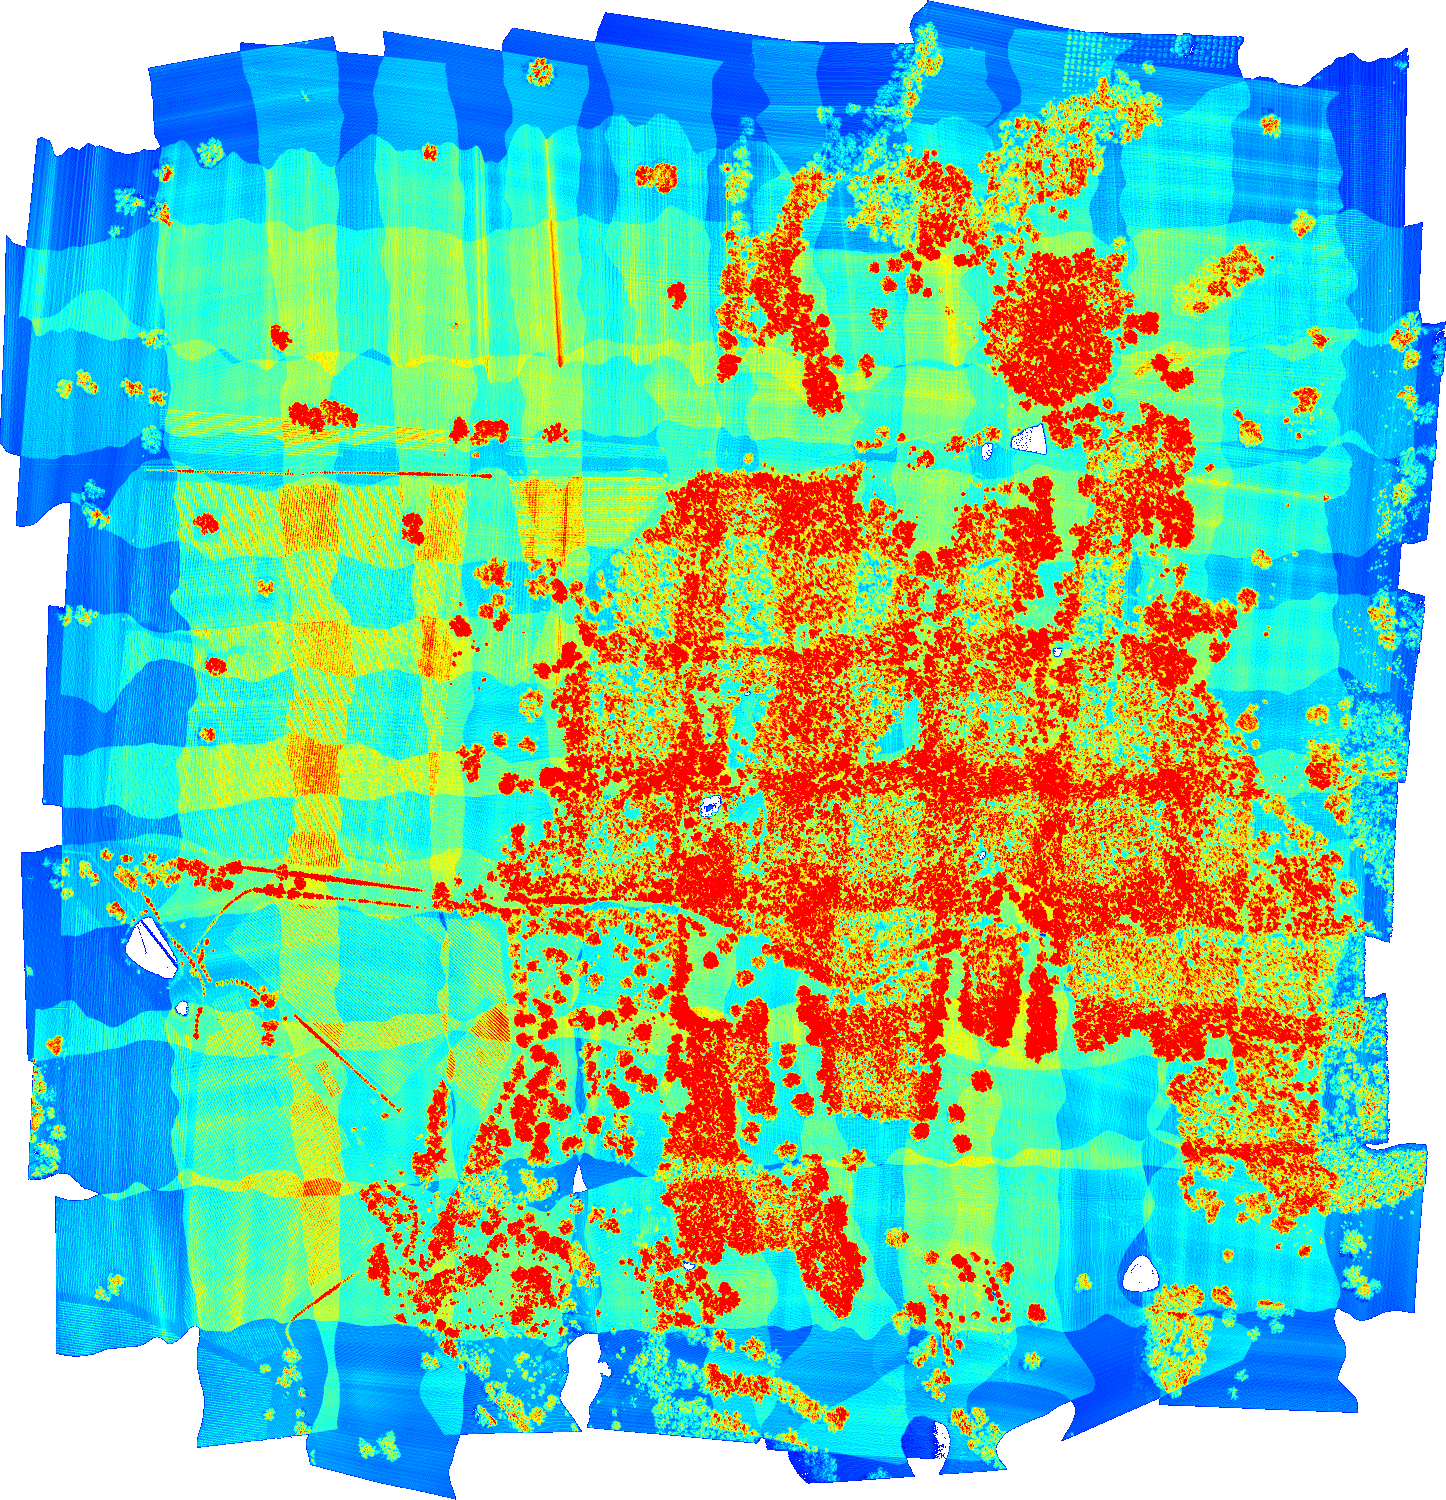
\includegraphics[width=0.45\textwidth]{images/densidad}
    \end{center}
  }

  \only<4>{Densidad de pasadas
    \begin{center}
      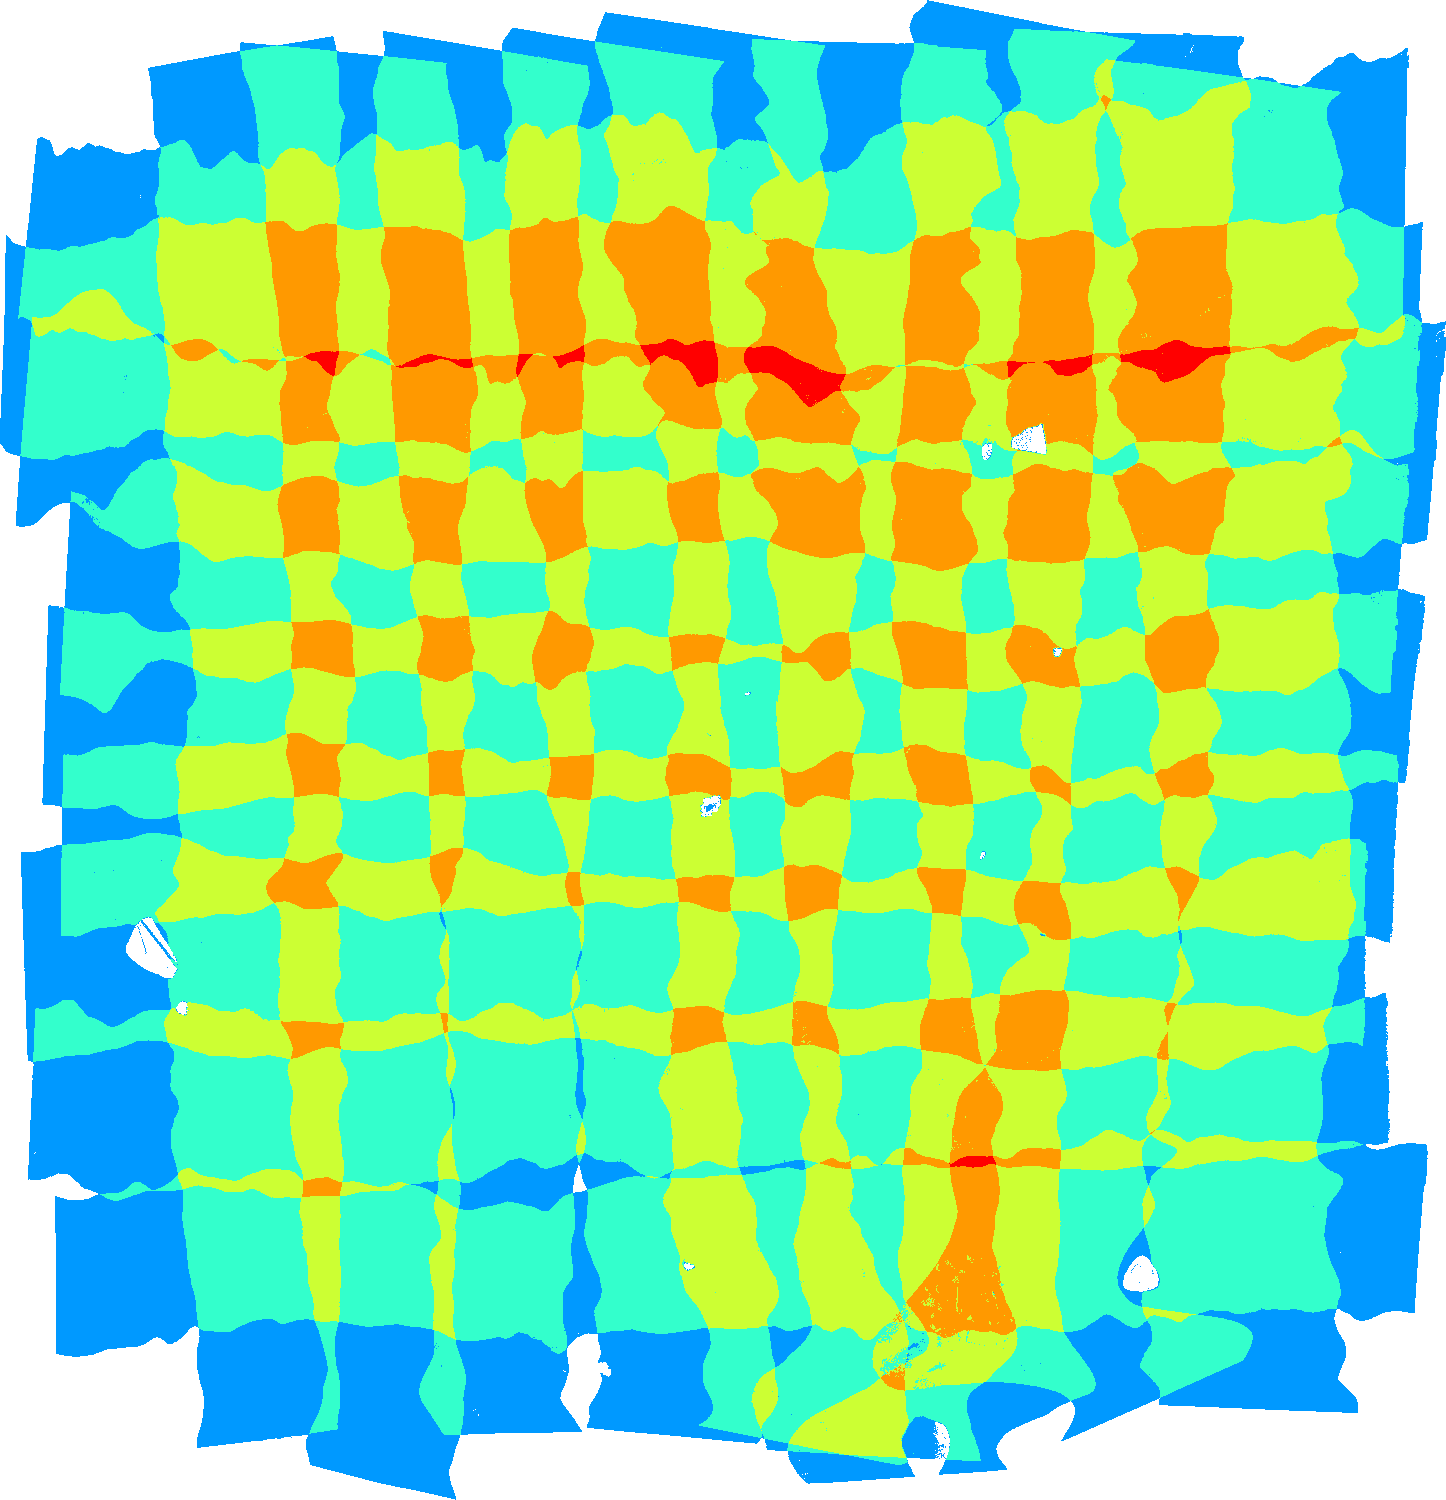
\includegraphics[width=0.45\textwidth]{images/densidad_pasadas}
    \end{center}
  }
\end{frame}
%%==================================================================F
\begin{frame}
  \frametitle{Calidad de los datos}
  \begin{enumerate}
    \item<1-> Información sobre la consistencia de los datos
    \item<2-> ¿La calidad del filtro? (terreno vs. no-terreno)
      \begin{itemize}
        \item Introducen errores en zonas complejas
        \item No hay un modo preciso de calcular la calidad de la clasificación
        \item Suelen estar basado en la \emph{\alert{experiencia práctica}}
      \end{itemize}
    \item<3-> Vegetación baja
      \begin{itemize}
        \item Dificil decir si un eco pertenece al terreno
        \item Introducen un \alert{sesgo sistemático} en altura
        \item Se necesitan información adicional
      \end{itemize}
  \end{enumerate}
\end{frame}
%%==================================================================F
\begin{frame}
  \frametitle{Calidad del modelo}
  \begin{enumerate}
    \item<1-> Calidad \alert<1>{interior}
      \begin{itemize}
        \item Es la calidad del modelo respecto a las \alert<1>{propios datos}
      \end{itemize}
    \item<2-> Calidad \alert<2>{exterior}
      \begin{itemize}
        \item Es la calidad del modelo respecto a \alert<1>{puntos de control
          externos (GCP)}
      \end{itemize}
  \end{enumerate}
\end{frame}
%%==================================================================F
\begin{frame}
  \frametitle{Calidad interior}
  \begin{enumerate}
    \item<1-> Es la calidad del modelo respecto a las propios datos
    \item<2-> Se aplica la ley propagación de los errores
    \item<2-> \alert<2>{RMSE} (raíz del error cuadrático medio)
      \[ \mathrm{RMSE(\widehat\theta)}=\sqrt{\mathrm{E}\left[(\widehat\theta - \theta)^2\right]}\]
    \item<3-> Representa la precisión del proceso de generación del DTM 
    \item<3-> Ayuda a identificar áreas con diferencias significativas entre
      modelo y datos
  \end{enumerate}
\end{frame}
%%==================================================================F
\begin{frame}
  \frametitle{Calidad exterior}
  \begin{enumerate}
    \item<1-> Es la calidad del modelo respecto a puntos de control externos (GCP)
      \begin{itemize}
        \item Los GCP no tienen que usarse durante la generación del DTM
        \item Tienen que ser mucho más precisos que los datos de input
      \end{itemize}
    \item<2-> Describe tanto los inputs como el proceso del modelado
    \item<2-> Generalmente se utiliza \alert<2>{RMSE}
    \item<3-> Estimación en \alert{altura} [Karel y Kraus (2006)]
        \[\sigma_z[\mathrm{cm}] = \pm\left(\dfrac{6}{\sqrt{n}} +
        30\tan(\alpha)\right)\]
      \begin{itemize}
        \item $n$: densidad puntual (pts/m$^2$)
        \item $\tan(\alpha)$: inclinación del terreno
      \end{itemize}
  \end{enumerate}
\end{frame}
%%==================================================================Sc
\subsection{Reducción de los datos}
%%==================================================================F
\begin{frame}
  \frametitle{Densidad puntual}
  \begin{enumerate}
    \item \alert{Todavía} es importante una reducción de la densidad
      puntual\alert{!}
    \item Escaneo: $100$ KHz $\Rightarrow$ \alert{$\approx$ 10
      pts/$\mathrm{m}^2$} $\Rightarrow$ Alta resolución en el DTM
    \item Problemas de almacenamiento y procesado
    \item Necesaria una reducción de la densidad
    \item Métodos
      \begin{itemize}
        \item Cambio de la estructura del DTM
        \item Sin cambio de la estructura del DTM
      \end{itemize}
  \end{enumerate}
\end{frame}
%%==================================================================F
\begin{frame}
  \frametitle{Remuestreo}
  \begin{enumerate}
    \item Métodos estándar en el procesado de imágenes digitales
    \item Menor resolución con celdas más grandes
    \item El valor del píxel nuevo se deriva de las celdas originales
    \item<2-> \alert<2>{Ventajas}
      \begin{itemize}
        \item Aplicable también para mallas
        \item Muy rápido y mantiene la estructura
      \end{itemize}
    \item<3-> \alert<3->{Desventajas}
      \begin{itemize}
        \item No son adaptativos: presentan problemas con diferencia de alturas
         \begin{itemize}
           \item<4-> Raster adaptativos locales\only<5>{: \alert{poco usados}}
         \end{itemize}
      \end{itemize}
  \end{enumerate}
\end{frame}
%%==================================================================F
\begin{frame}
  \frametitle{TIN's}
  \begin{enumerate}
    \item \alert<1-3>{Purga de puntos}
      \begin{itemize}
        \item<2-> Considera el TIN completo 
        \item<3-> elimina puntos paso a paso
      \end{itemize}
    \item \alert<4-5>{Aproximación por subdivisión}
      \begin{itemize}
        \item<4-> Empieza con un TIN aproximado
        \item<5-> Utiliza algoritmos \alert<5>{divide y vencerás} hasta alcanzar cierto
          criterio
      \end{itemize}
    \item<6-> Necesitan teselar el TIN 
    \item<7-> Poco eficaces \alert<7>{justo después} del filtrado
      \begin{itemize}
        \item Errores en las observaciones y en zonas de solape (poco eficaces)
        \item Interpolación suavizada de alta resolución de los puntos
      \end{itemize}
  \end{enumerate}
\end{frame}
%%==================================================================Sc
\section{Clasificación mediante splines}
%%==================================================================Sb
\begin{frame}
  \frametitle{Objetivos y metodología}
  \begin{enumerate}[<+->]
    \item Objetivo
    \begin{itemize}
       \item Generar un DTM, un modelo de \alert<2>{vegetación}, un modelo de
         \alert<2>{edificios}...
    \end{itemize}
    \item ¿Cómo?
    \begin{itemize}
      \item Interpolación de \alert<4>{superficies} mediante un ajuste de mínimos
            cuadrados de splines utilizando una norma de Tychonov
          \item Estudio de pendientes: \alert<5>{Morfología}
          \item \alert<6>{Segmentación} de objetos
    \end{itemize}
  \end{enumerate}
\end{frame}
%%==================================================================Sb
\subsection{Splines}
%%==================================================================F
\begin{frame}
    \frametitle{Spline bilineares y bicúbicas}
    \begin{center}
        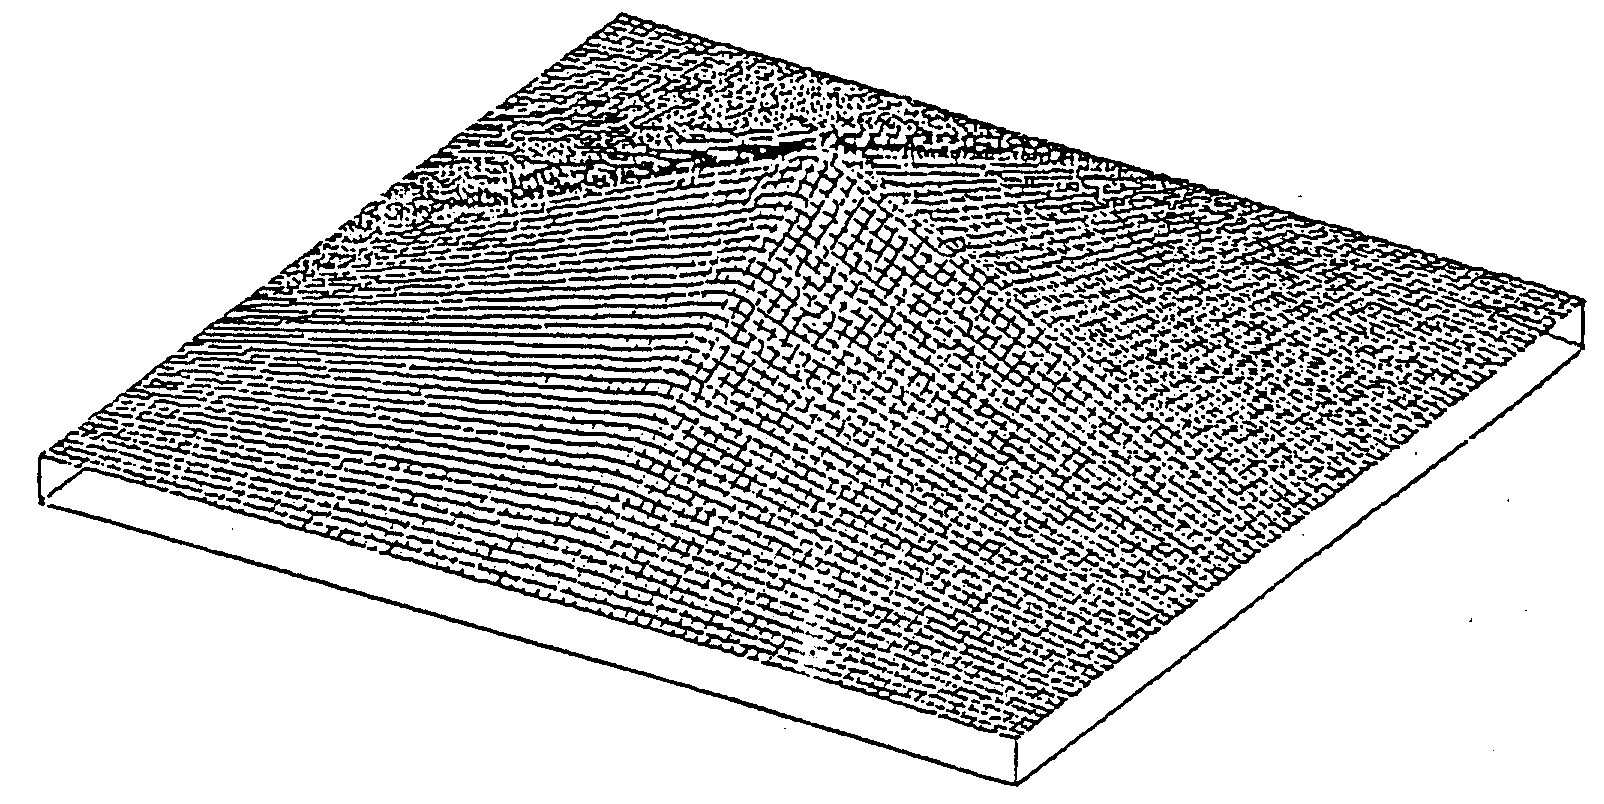
\includegraphics[width=0.45\textwidth]{images/bilinear_spline.jpg}
        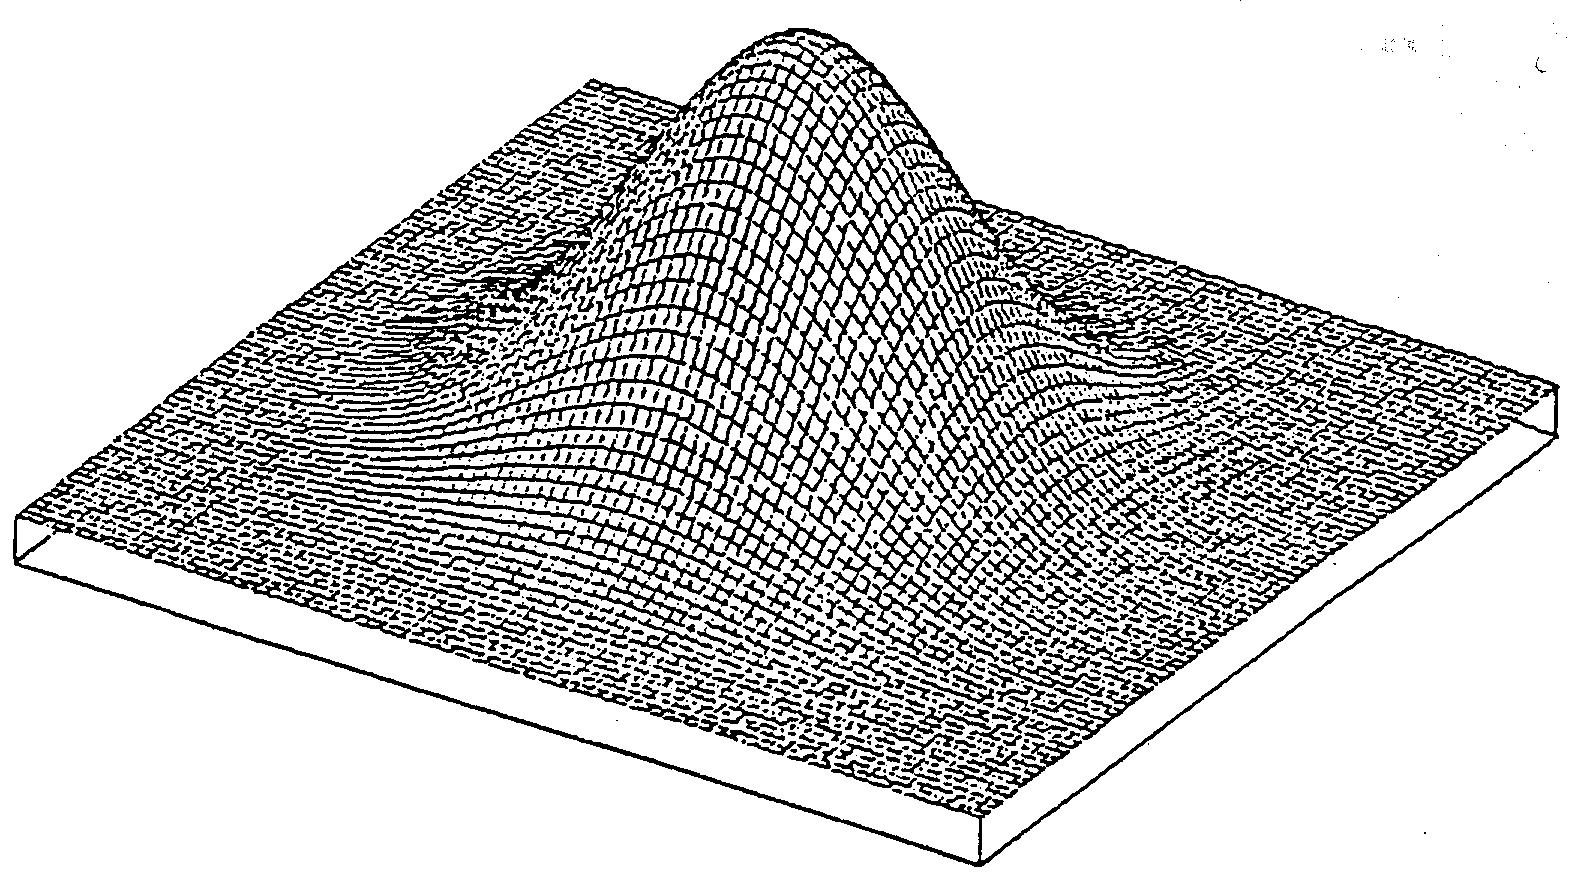
\includegraphics[width=0.45\textwidth]{images/bicubic_spline.jpg}
        %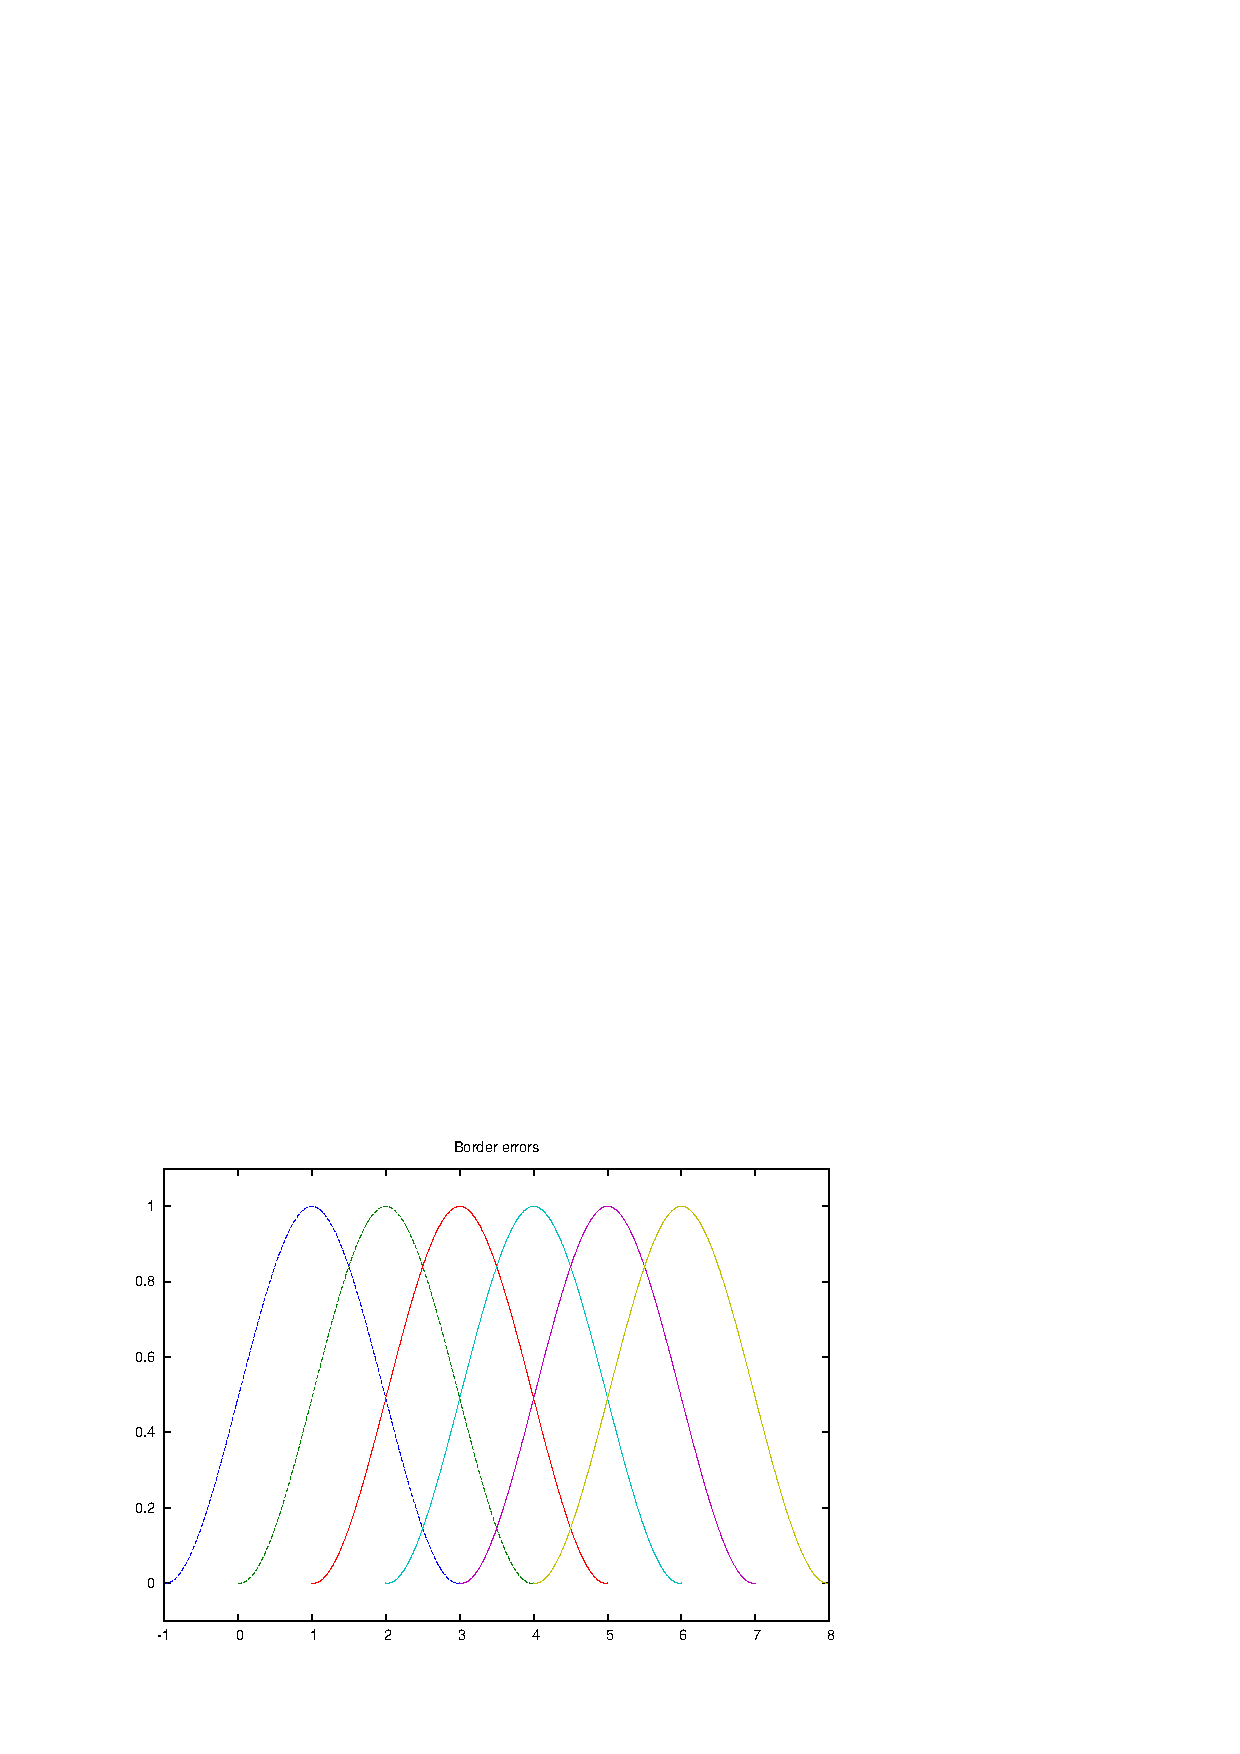
\includegraphics[width=0.45\textwidth]{images/border_errors.jpg}
    \end{center}
\end{frame}
%%==================================================================Sb
\subsection{Puntos groseros}
%%==================================================================F
\begin{frame}
   \frametitle{Puntos groseros}
   \begin{enumerate}
    \item Hay siempre puntos anómalos debido a diferentes eventos:
     \begin{itemize}
 	\item<2-> \alert<2,3,6>{Pájaros}
 	\item<4-> \alert<4,6>{Nubes de agua}
 	\item<5-> \alert<5,6>{``Multipath''}...
     \end{itemize}
    \item<6>{\alert<6>{\textexclamdown\textexclamdown Deben ser eliminados!!}} 
   \end{enumerate}
   \begin{picture}(0,100)
       \uncover<2>{\put(10,10){
\includegraphics[height=30mm]{images/angry_birds}}}     
       \uncover<3,6>{\put(10,10){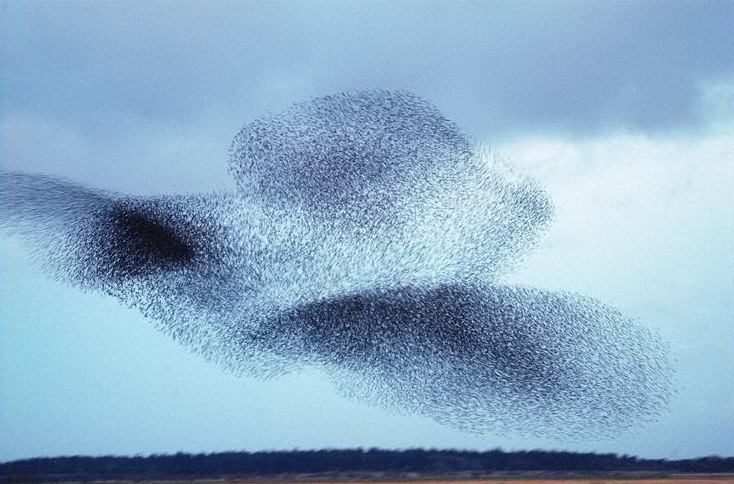
\includegraphics[height=30mm]{images/bandada}}}
       \uncover<4>{\put(50,10){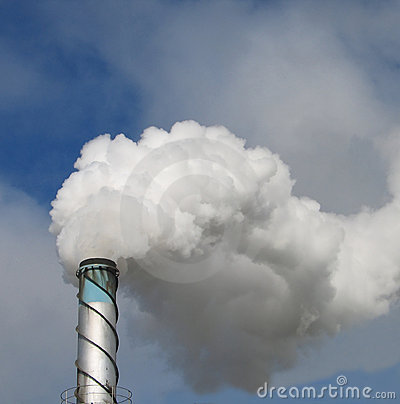
\includegraphics[height=30mm]{images/vapor_chimenea}}}
       \uncover<4,6>{\put(150,10){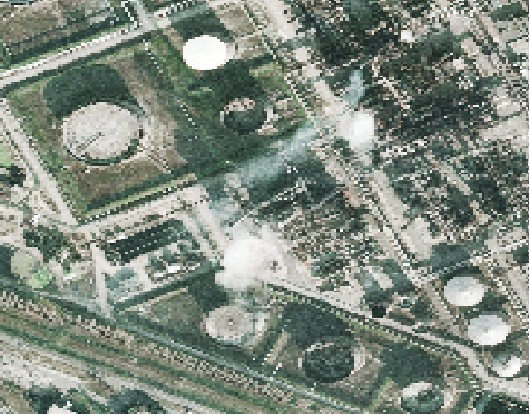
\includegraphics[height=30mm]{images/fumo}}}
       \uncover<5,6>{\put(280,10){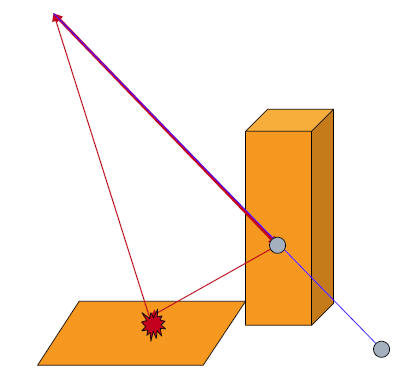
\includegraphics[height=30mm]{images/multipath}}}
    \end{picture}
\end{frame}
%%==================================================================F
\begin{frame}
   \frametitle{Detección de puntos groseros}
   \begin{itemize}
    \item<1-> La eliminación se hace mediante una interpolacion con splines 
        bicúbicas bastante lisa y baja resolución.
    \item<8-> Aquellos puntos que se alejen más de un umbral determinado son 
        considerados como puntos groseros y eliminados.
    \item<9-> El umbral por defecto son \alert<8>{$50~m$}
   \end{itemize}

    \begin{picture}(0,100)
       \only<2>{\put(80,0){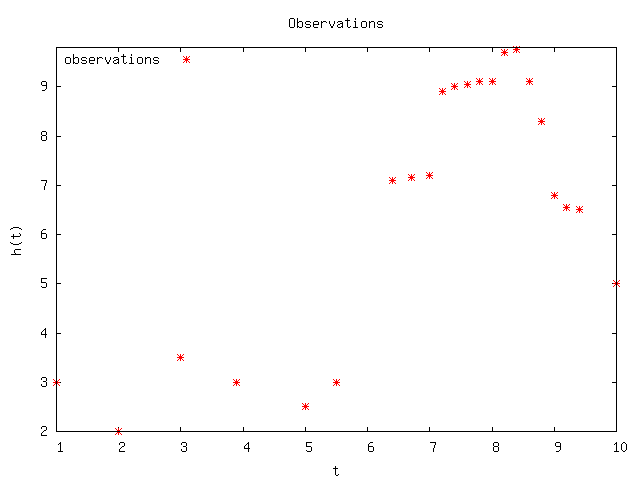
\includegraphics[height=35mm]{images/obs_splines}}}
       \only<3,8->{\put(80,0){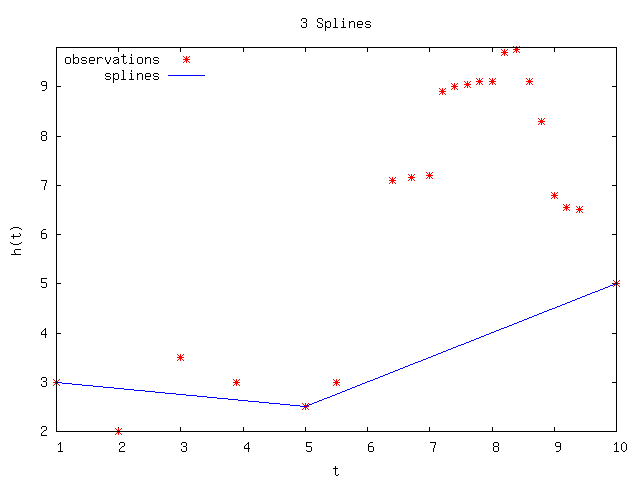
\includegraphics[height=35mm]{images/3splines}}}
       \only<4>{\put(80,0){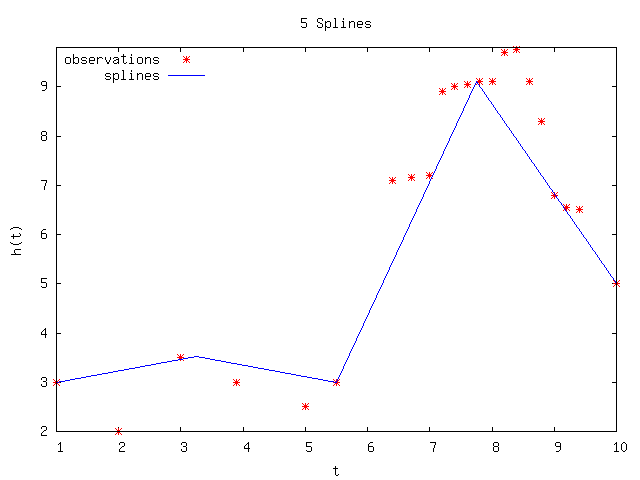
\includegraphics[height=35mm]{images/5splines}}}
       \only<5>{\put(80,0){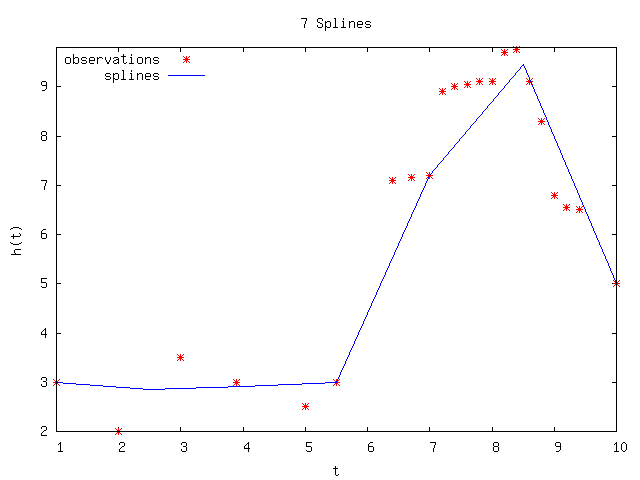
\includegraphics[height=35mm]{images/7splines}}}
       \only<6>{\put(80,0){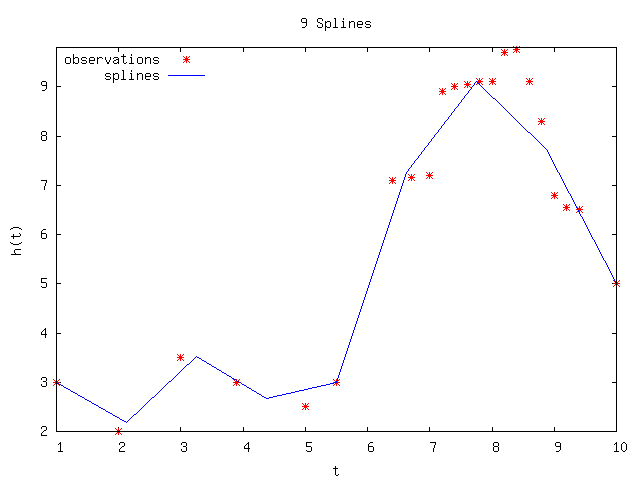
\includegraphics[height=35mm]{images/9splines}}}
       \only<7>{\put(80,0){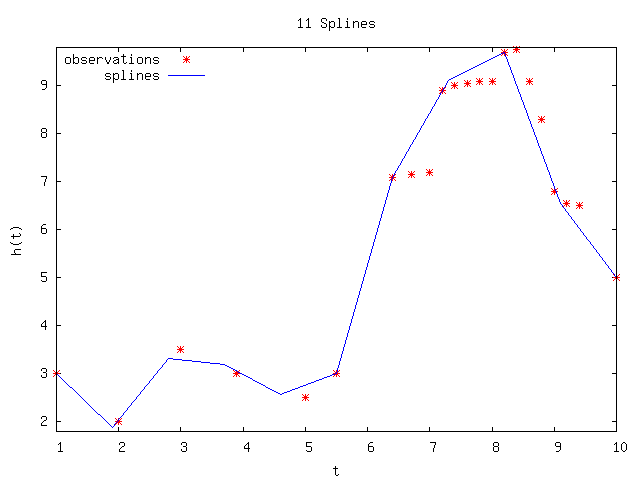
\includegraphics[height=35mm]{images/11splines}}}
    \end{picture}
\end{frame}
%%==================================================================Sb
\subsection{Detección de bordes}
%%==================================================================F
\begin{frame}
  \frametitle{Detección de bordes}
\begin{beamerboxesrounded}[shadow=true]{Definición: \emph{Borde}}
     \alt<1>{\alert<1>{NO} es un señor antipático $\Rightarrow$ \alert<1>{NO} 
        es tu jefe}{Es una fuerte variación en altura correspondiente a una 
        pequeña variación en planimetría}
    \end{beamerboxesrounded}

\only<2>{
  \begin{picture}(0,100)
    %\centering
    \begin{tikzpicture}[scale=0.7]
    \draw[thick] (-5,0) -- (2.5,0);
    \filldraw[black!20!white] (-2,0) -- (-2,2) -- (0,3) -- (2,2) -- (2,0) -- cycle;
    \draw (-2,0) -- (-2,2) -- (0,3) -- (2,2) -- (2,0) -- cycle;

    \coordinate[mark coordinate] (S) at (-2,0);
    \coordinate[mark coordinate] (B) at (-2,2);
    \node[anchor=south east] at (S){};
    \node[anchor=north west] at (B){};
    \node[anchor=west] at (-1,1){Objeto};
    \end{tikzpicture}
  \end{picture}
  \begin{picture}(0,100)
     \uncover<2>{\put(200,-5){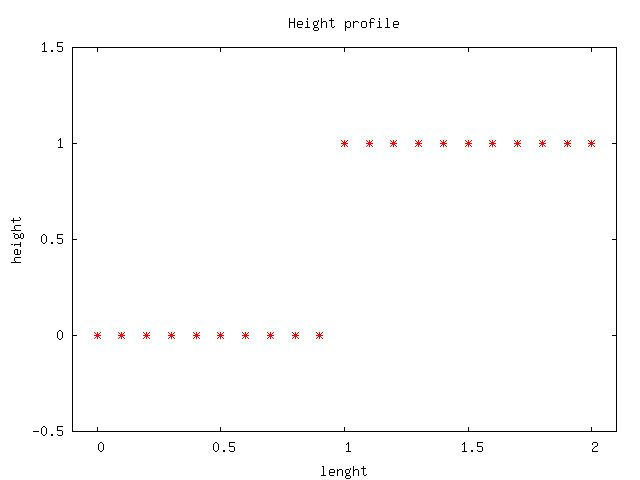
\includegraphics[height=30mm]{images/height_edge}}}
  \end{picture}
}
\begin{enumerate}
 \item<3-> El análisis de bordes no es fácil porque los puntos no están distribuidos regularmente
 \item<4-> Se pueden regularizar los puntos $\Rightarrow$ se rasteriza: 
    \begin{itemize}
        \item<4-> \alert<4>{mínimo} y \alert<4>{máximo}
	\item<5-> \alert<5>{Media}
	\item<6-> \alert<6>{Interpolación}
	\item<7-> \alert<7>{\emph{kriging}}...
    \end{itemize}
  \item<8-> \alert<8>{Pérdida de información} altimétrica
\end{enumerate}
\end{frame}
%%==================================================================F
\begin{frame}
  \frametitle{Cálculo de bordes}
\begin{enumerate}
  \item Se trabaja con una interpolación con spline bilineares que se ajuste 
    mucho a las observaciones (nuestros puntos)
  \item<2->{Para esta superficie se calcula:}
\begin{itemize}
 \item<2-> El \alert<2>{Gradiente} para cada punto: $G_m = \sqrt{G_x^2 + G_y^2} = \sqrt{\left( \dfrac{dz}{dx}\right)^2 + \left( \dfrac{dz}{dy}\right)^2}$
 \item<3-> La \alert<3>{dirección normal}: $\vartheta_P = \arctan\left(\dfrac{G_y}{G_x} \right)$
\end{itemize}
\end{enumerate}

  \uncover<4->{\alert<4>{Estos dos parámetros no son suficientes!!}}
\end{frame}
%%==================================================================F
\begin{frame}
  \frametitle{Valor gradiente}
  \begin{enumerate}[<+->]
   \item El gradiente tiene un valor muy alto en el borde de los objetos pero también el punto exterior más próximo
   \item Debido al ruido en las observaciones, el valor más alto del gradiente \alert<2>{puede ser el equivocado}
  \end{enumerate}
    \begin{picture}(0,110)
        \only<1>{\put(80,0){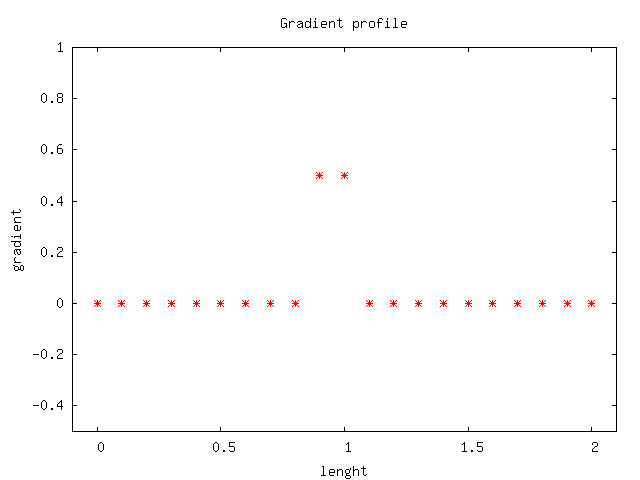
\includegraphics[height=40mm]{images/gradient_edge}}}
        \only<2>{\put(80,0){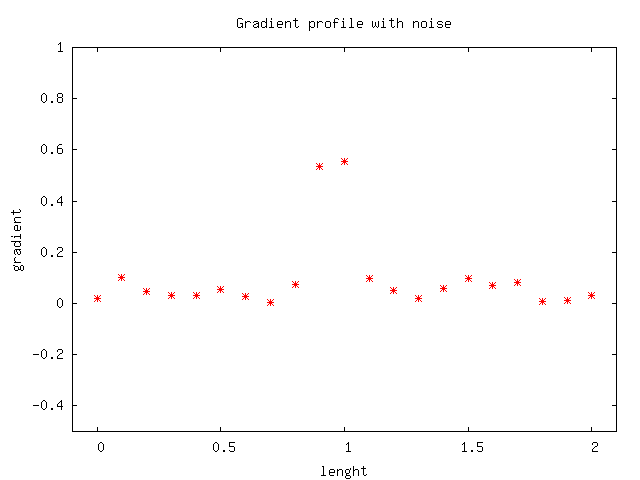
\includegraphics[height=40mm]{images/gradient_noise_edge}}}
    \end{picture}
\end{frame}
%%==================================================================F
\begin{frame}
  \frametitle{Cálculo de residuos}%
  \begin{enumerate}[<+->]%
   \item Se trabaja con una interpolación con spline bicúbicas con resolución muy baja 
       para obtener una \alert<1>{superficie muy lisa}%
   \item Se calcula el residuo entre la superficie y las observaciones%
   \item El punto con residuo positivo será nuestro punto \alert<3>{borde} %
  \end{enumerate}%
\uncover<3->{
  \begin{figure}[!b]
    \centering
    \begin{tikzpicture}[scale=0.85]
    %\includegraphics[height=50mm]{images/figure_6}
    \draw[thick] (-5,0) -- (3,0);
    \filldraw[black!20!white] (-2,0) -- (-2,2) -- (0,3) -- (2,2) -- (2,0) -- cycle;
    \draw (-2,0) -- (-2,2) -- (0,3)node[above]{Objeto} -- (2,2) -- (2,0) -- cycle;
    \draw[thick] (-4.5,0.3)node[above]{Interpolaci\'on} -- 
        (-3.5,0.3) .. controls (-1.5,.4) and (-1.5,2) .. (0,2);

    \coordinate[mark coordinate] (N) at (-2,0);
    \coordinate[mark coordinate] (P) at (-2,2);
    \node[anchor=south east] at (N){--};
    \node[anchor=north west] at (P){+};

    \node[anchor=west] at (-0.5,1){+ Borde};
    \node[anchor=west] at (-0.5,0.5){-- \  Terreno};
    \end{tikzpicture}
  \end{figure}
}
\end{frame}
%%==================================================================F
\begin{frame}
  \frametitle{Identificación final de bordes}%
  Para que un punto sea considerado como el borde de un objeto se debe cumplir:
  \begin{enumerate}[<+->]%
	\item El gradiente debe ser mayor que un cierto umbral dado por el usario
	\item Si el gradiente es grande pero \alert<2>{sin} llegar al umbral, además se debe verificar que:
	\begin{itemize}
	 \item El residuo es \alert<3>{positivo}
	 \item La dirección normal no se desvía mas de un valor dado.
	\end{itemize}
  \end{enumerate}
\end{frame}
%%==================================================================Sb
\subsection{Region Growing}
%%==================================================================F
\begin{frame}
  \frametitle{``Region Growing''}
\begin{beamerboxesrounded}[shadow=true]{Hipótesis}
El interior del objeto será siempre igual o más alto que los bordes (su altura media)
\end{beamerboxesrounded}

\begin{enumerate}
 \item El objetivo en este paso es reconocer el \alert{interior} de los objetos
 \item Para cada borde se construye un \alert{conj. convexo} y en su interior se ejecuta un algoritmo de \alert{\emph{region growing}} para verificar la hipótesis
\end{enumerate}
\end{frame}
%%==================================================================F
%\begin{frame}
%  \frametitle{``Region Growing''}
%\begin{figure}[t]
% \begin{center}
%\tiny
%  \begin{tikzpicture}[scale=0.2, node distance=1.25cm, auto]
%    % Region growing
%    \node[io] (semilla) {Elegir Semilla};
%    \node[block, below of=semilla] (este) {Moverse a celda Este};
%    \node[decision, below of=este] (visitadaE) {¿Visitada?};
%    \node[block, below of=visitadaE, node distance=1cm] (norte) 
%        {Moverse a celda Norte};
%    \node[decision, below of=norte] (visitadaN) {¿Visitada?};
%    \node[block, below of=visitadaN, node distance=1cm] (visitada) 
%        {Marcar como visitada};
%    \node[block, right of=visitada, node distance=2cm] (retroceder) {Retroceder};
%    \node[decision, right of=visitadaE, node distance=1.5cm] (valor1E) 
%        {¿Valor = 1?};
%    \node[decision, left of=visitadaN, node distance=1.5cm] (valor1N) 
%        {¿Valor = 1?};
%    \node[decision, above of=retroceder] (EsSemilla) {¿Es la semilla?};
%    \node[io, right of=EsSemilla, node distance=1.5cm] (convhull) 
%        {Crear soporte compacto};
%
%    % Flujo
%    \path[line] (semilla) -- node{}(este);
%    \path[line] (este) -- node{}(visitadaE);
%    \path[line] (visitadaE) -- node{si}(norte);
%    \path[line] (visitadaE) -- node{no}(valor1E);
%    \path[line] (valor1E) |- node[near start]{si}(este);
%    \path[line] (valor1E) |- node[near start]{no}(norte);
%    \path[line] (norte) -- node{}(visitadaN);
%    \path[line] (visitadaN) -- node{si}(visitada);
%    \path[line] (visitadaN) -- node{no}(valor1N);
%    \path[line] (valor1N) |- node[near start]{si}(este);
%    \path[line] (valor1N) |- node[near start]{no}(visitada);
%    \path[line] (visitada) -- node{}(retroceder);
%    \path[line] (retroceder) -- node{}(EsSemilla);
%    \path[line] (EsSemilla) -- node[near start]{si}(convhull);
%    \path[line] (EsSemilla) |- node[near start]{no}(este);
%    \path[line] (convhull) |- node{}(semilla);
%  \end{tikzpicture}
% \end{center}
%\end{figure}
%\end{frame}
%%==================================================================F
\begin{frame}
  \frametitle{Primera clasificación}
Los puntos viene clasificados por su posición con respecto al terreno: \pause
\begin{enumerate}
 \item \alert{Objeto}: Si están dentro del conj. convexo y su altura es mayor que la altura media del borde
 \item \alert{Terreno}: En cualquier otro caso.
\end{enumerate}

\pause
Y por el tipo de impulso:
\begin{enumerate}
 \item \alert{\'Unico impulso}: Si solo se ha recibido un eco de ese punto
 \item \alert{Doble impulso}: Si se han recibido más impulsos
\end{enumerate}
\end{frame}
%%==================================================================Sb
\subsection{Corrección}
%%==================================================================F
\mode<beamer>{
  \pgfdeclareimage[width=0.4\textwidth]{fumo}{images/fumo}
  \pgfdeclareimage[width=0.4\textwidth]{fumo}{images/google_techos}
}
\begin{frame}
  \frametitle{Errores en la clasificación}
  \begin{columns}
    \begin{column}{0.5\textwidth}
      \begin{enumerate}[<+->]
    	\item La hipótesis de las alturas falla
        \item Confusión de alturas
    	\item Se han identificado bordes pertenecientes al terreno pero no a objetos
     \end{enumerate}
    \end{column}
   \begin{column}{0.45\textwidth}
   \begin{figure}[h!]
   \centering
      \only<1>{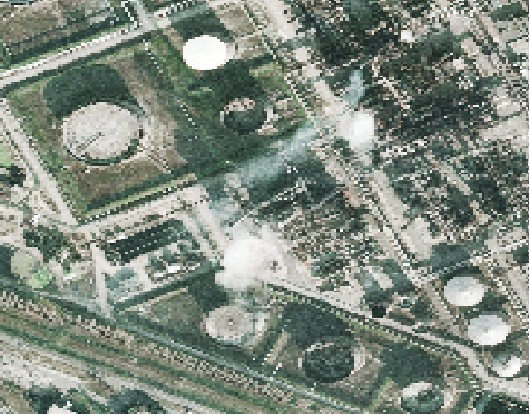
\includegraphics[height=40mm]{images/fumo}}
      \only<2>{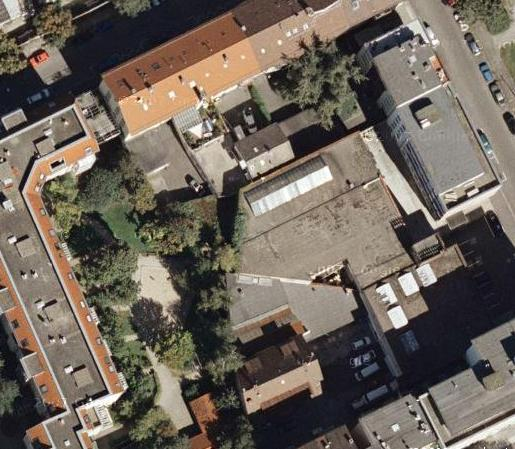
\includegraphics[height=40mm]{images/google_techos}}
      \only<3>{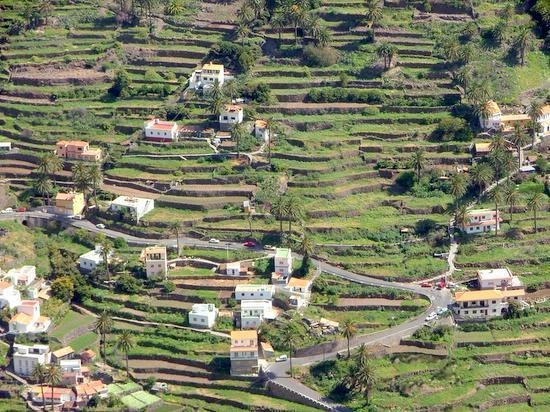
\includegraphics[height=40mm]{images/terrazas}}
   \end{figure}
   \end{column}
  \end{columns}
\end{frame}
%%==================================================================F
\begin{frame}
  \frametitle{Corrección final}
Se utilizan los puntos \alert<1>{Terreno único impulso} para realizar una
interpolación con splines bilineares y resolucion baja para obtener una
superficie bastante lisa.
  \begin{minipage}{0.5\textwidth}
    \begin{enumerate}
      \item<2-> Si un punto terreno está lo suficientemente alejado de la superficie se reclasifica como \alert<2>{objeto}
      \item<3-> Si un punto objeto está lo suficientemente cercano a la superficie se reclasifica como \alert<3>{terreno}
    \end{enumerate}
  \end{minipage}%
  ~%
  \begin{minipage}{0.45\textwidth}
   \begin{figure}[h!]
   \centering
      \uncover<2->{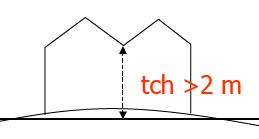
\includegraphics[height=20mm]{images/correct_objeto}}
      \uncover<3->{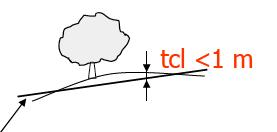
\includegraphics[height=20mm]{images/correct_terreno}}
   \end{figure}
  \end{minipage}
\end{frame}
%%==================================================================Sb
\subsection{Vegetación}
%%==================================================================F
\begin{frame}
  \frametitle{Motivaciones}
  \begin{enumerate}[<+->]
    \item El filtro anterior clasifica entre \alert{terreno} Vs. \alert{objeto}: 
  \begin{itemize}[<+->]
    \item Participó en el test del ISPRS: Buenos resultados
    \item Incompleta: \alert<3>{NO distingue vegetación}
  \end{itemize}
    \item Detectar vegetación en una nube ALS es importante para
      \uncover<4->{\alert{estudios hidrológicos}},
      \uncover<5->{\alert{modelización urbana},} \uncover<6->{\alert{estudios
      forestales}, etc\ldots}
    \item Desarrollo del filtro de vegetación porque:
    \begin{itemize}
    \item<7-> Existe ya una estructura adecuada de datos
    \item<7-> Dado que está bajo licencia libre, su publicación también deberá ser
      libre
    \item<7-> Completar el algoritmo que participó en el ISPRS
    \end{itemize}
  \end{enumerate}
\end{frame}
%%==================================================================F
\begin{frame}
  \frametitle{Clasificación de vegetación}
  \begin{enumerate}
    \item<1-> Los datos de partida son los clasificados como terreno u objecto
    (tanto único como doble impulso).
    \item<2-> Se crea una máscara ráster.
    \item<3-> Podemos buscar:
      \begin{enumerate}
        \item<3-> \alert<3>{Edificios}
          \begin{itemize}
            \item valor celda = 1 si al menos un punto ``objeto único impulso''
              cae en ella.
            \item valor de celda = 0 en otro caso
          \end{itemize}
        \item<4-> \alert<4>{Vegetación}
          \begin{itemize}
            \item valor celda = 1 si al menos un punto ``terreno doble impulso''
              cae en ella.
            \item valor de celda = 0 en otro caso
          \end{itemize}
      \end{enumerate}
  \end{enumerate}
\end{frame}
%%==================================================================F
\begin{frame}
  \frametitle{Clasificación de vegetación}
  \begin{enumerate}
    \item<1-> Se aplica un algoritmo de ``region growing'' a la mascara raster
        para crear conj. convexos. 
      \item<2-> Las \alert<2>{dimensiones} y la relación \alert<2>{área/perímetro}
        se usan para la clasificación de los segmentos:
    \begin{itemize}
        \item Objetos pequeños o muy estrechos no son edificios
        \item Puntos ``terreno doble impulso'' son considerados como vegetación
        \item Puntos ``objeto doble impulso'' fuera de los segmentos son
          considerados como vegetación
        \item El resto siempre es considerado edificio
    \end{itemize}
  \end{enumerate}
\end{frame}
%%==================================================================F
\begin{frame}
  \frametitle{Árbol de clasificación del filtro vegetación}
\begin{figure}[t!]
\begin{center}
\scriptsize
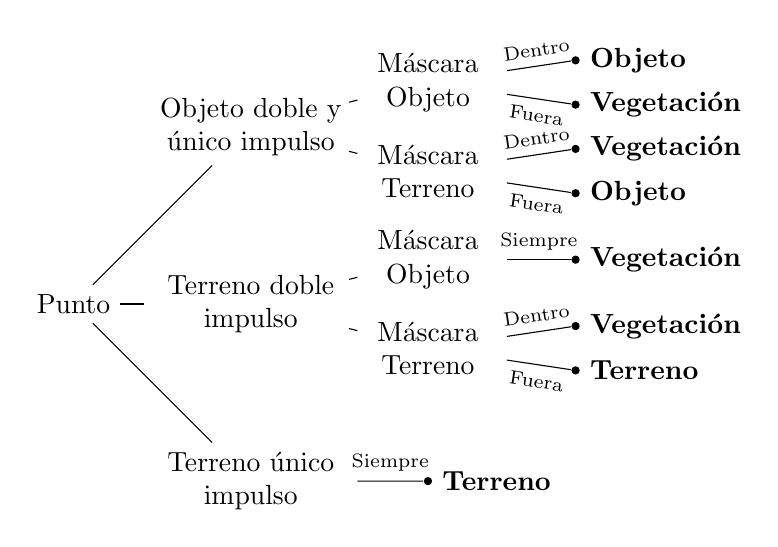
\begin{tikzpicture}[scale=0.75,grow=right, sloped,
    level 1/.style={sibling distance = 3cm, level distance = 3cm}, 
    level 2/.style={sibling distance = 1.5cm, level distance = 3cm},
    level 3/.style={sibling distance = 0.75cm, level distance = 2.5cm},
    punto/.style={text width=7em, text centered},
    mascara/.style={text centered, text width=5em},
    end/.style={circle, minimum width=3pt,fill, inner sep=0pt}]
  \node {Punto}
    child{ node[punto] {Terreno único impulso} 
       child{ node [end, label=right:{\textbf{Terreno}}] {}
              edge from parent node[above] {\scriptsize{Siempre}}
       }
    }
    child{ node[punto] {Terreno doble impulso}
       child{ node[mascara] {Máscara Terreno} 
          child{ node [end, label=right:{\textbf{Terreno}}] {}
                 edge from parent node[below] {\scriptsize{Fuera}}
          }
          child{ node [end, label=right:{\textbf{Vegetación}}] {}
                 edge from parent node[above] {\scriptsize{Dentro}}
          }
       }
       child{ node[mascara] {Máscara Objeto}
          child{ node [end, label=right:{\textbf{Vegetación}}] {}
                 edge from parent node[above] {\scriptsize{Siempre}}
          }
       }
    }
    child{ node[punto] {Objeto doble y único impulso}
       child{ node[mascara] {Máscara Terreno} 
          child{ node [end, label=right:{\textbf{Objeto}}] {}
                 edge from parent node[below] {\scriptsize{Fuera}}
          }
          child{ node [end, label=right:{\textbf{Vegetación}}] {}
                 edge from parent node[above] {\scriptsize{Dentro}}
          }
       }
       child{ node[mascara] {Máscara Objeto}
          child{ node [end, label=right:{\textbf{Vegetación}}] {}
                 edge from parent node[below] {\scriptsize{Fuera}}
          }
          child{ node [end, label=right:{\textbf{Objeto}}] {}
                 edge from parent node[above] {\scriptsize{Dentro}}
          }
       }
    }
;
\end{tikzpicture}
\caption{Árbol de decisión para la clasificación de los puntos en terreno,
vegetación y edificio.}
\label{fig:decision_tree}
\end{center}
\end{figure}
\end{frame}
%%==================================================================F
\begin{frame}
  \frametitle{Clasificación de la vegetación}
  \begin{minipage}{0.45\textwidth}
    \begin{figure}[h!]
      \centering
      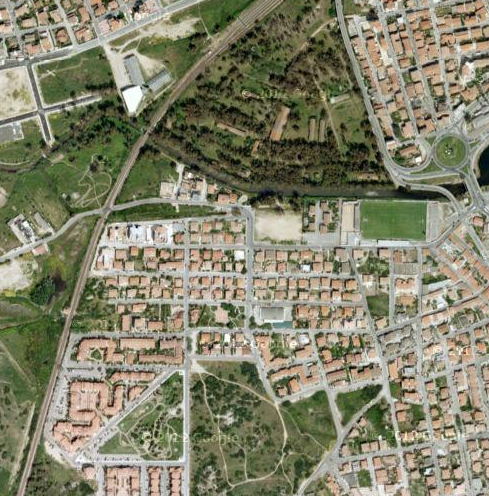
\includegraphics[width=0.95\textwidth]{images/olbia}
    \end{figure}
  \end{minipage}
  \begin{minipage}{0.45\textwidth}
    \begin{figure}[h!]
      \centering
      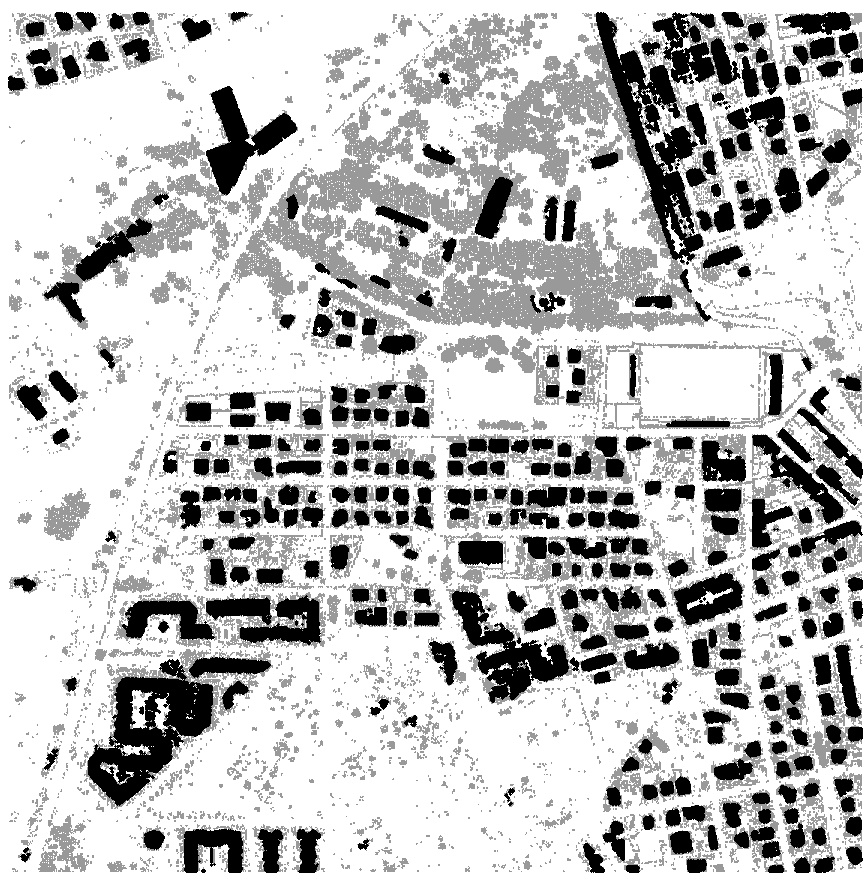
\includegraphics[width=0.95\textwidth]{images/olbia_veg_build}
    \end{figure}
  \end{minipage}
\end{frame}
%%==================================================================F
\begin{frame}
  \frametitle{Resultados}
  \begin{enumerate}[<+->]
    \item El filtro vegetación está fuertemente afectado por el filtro terreno:
    \begin{itemize}
      \item Altos errores del tipo I (error de omisión) debido
        a bordes de edificios mal clasificados como vegetación.
      \item Errores de tipo II (error de comisión) debido
        a zonas de densa vegetación tomada como edificios o incluso zonas
        terreno clasificadas como objetos.
    \end{itemize}
    \item Alrededor del 90\% de los puntos se clasifican correctamente.
    \begin{itemize}
      \item Amplias zonas vegetales son correctamente clasificadas, así como la
        mayoría de árboles individuales. 
      \item La figura y forma de los eficios está siempre bien definida.
    \end{itemize}
  \end{enumerate}
\end{frame}
%%==================================================================F
\begin{frame}
  \frametitle{Resultados}
  \begin{itemize}[<+->]
    \item Errores de \alert<1>{tipo I} (descartar puntos edificio):
      \alert<1>{$16.6\%$}
    \item Errores de \alert<2>{tipo II} (Aceptar puntos vegetación como
      edificio): \alert<2>{$7.5\%$}
      \item \alert<3>{Error Total}: \alert<3>{$10.6\%$}
    \end{itemize} 
     \begin{table}[b!]
    \centering
    \begin{tabular}{lccccr}
      \multicolumn{6}{c}{\bfseries{Matriz de Confusión}} \\
      \hline
      \textbf{Clasif.} & \multicolumn{2}{c}{Edificios} & 
        \multicolumn{2}{c}{Vegetación} & Total \\
      \cline{2-6}
      \textbf{Verdad} & \multicolumn{2}{c}{Puntos (\%)} & 
        \multicolumn{2}{c}{Puntos (\%)} & Total \\
      \hline
      Edif. & \multicolumn{2}{c}{179678 (83.4)} & 
        \multicolumn{2}{c}{34919 (\alert<1>{16.6})} & 214597 \\
      Veg. & \multicolumn{2}{c}{37590 (\alert<2>{7.5})} & 
        \multicolumn{2}{c}{388709 (92.5)} & 426299 \\
      Total & \multicolumn{2}{c}{217268 (--)} & 
      \multicolumn{2}{c}{423628 (--)} & 640896\footnote{Las estadísticas están referidas a aquellos puntos con una pre-clasificación distinta de terreno único impulso} \\
      \hline
    \end{tabular}
    \end{table}
\end{frame}
%%==================================================================F
\begin{frame}
  \frametitle{Solapes}
  \begin{enumerate}
    \item<1-> Durante las interpolaciones, se divide toda la región en teselas
      solapadas
      \begin{itemize}
        \item<1-> Permite la computación de la interpolación de modo más rápido
        \item<2-> Elimina los problemas de alocación de memoria
      \end{itemize}
    \item<3-> En las zonas de solape
    \begin{itemize}
        \item<3-> Asegura la continuidad de toda la interpolación
        \item<4-> Introduce una discontinuidad en la primera derivada: Errores en el
          mapa de aspectos en zonas con ausencia de datos
      \end{itemize}
  \end{enumerate}
\end{frame}
%%==================================================================F
\begin{frame}
  \frametitle{Solapes}
    \begin{figure}[h!]
      \centering
      \only<1>{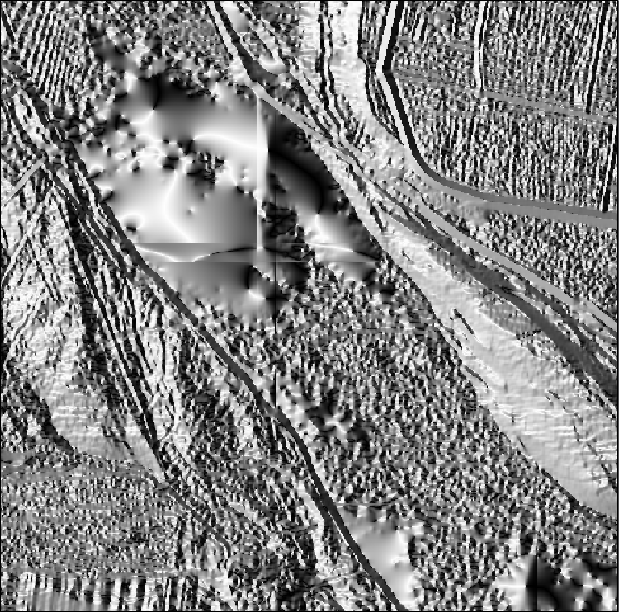
\includegraphics[width=0.65\textwidth]{images/errores_aspect}}
      \only<2>{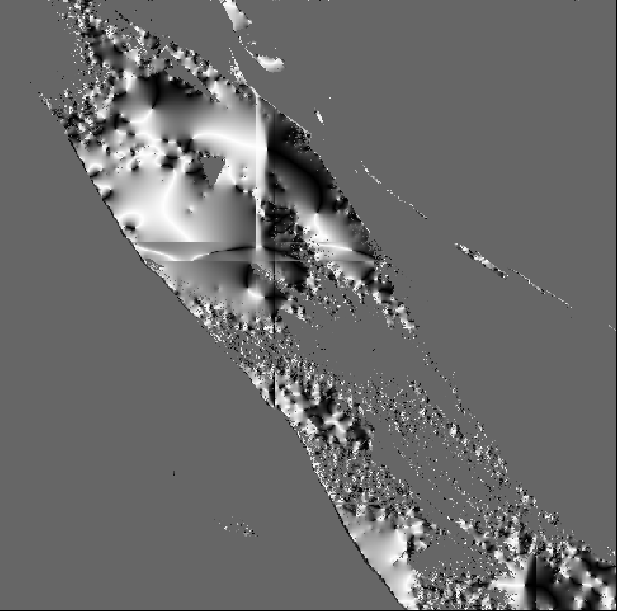
\includegraphics[width=0.65\textwidth]{images/errores_aspect_mascara}}
      \only<3>{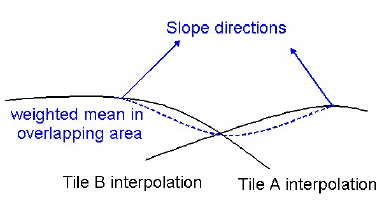
\includegraphics[width=0.65\textwidth]{images/error_interpolacion_solapes}}
    \end{figure}
\end{frame}
%%==================================================================F
%\begin{frame}
%  \frametitle{Computación}
%    \begin{table}[h!]
%      \centering
%    \begin{tabular}{ccrrr}
%    \toprule
%    \multicolumn{5}{c}{\bfseries Interpolación Bilinear} \\
%    \hline
%    \bfseries Paso de Spline & \bfseries Número de teselas & \bfseries
%    tradicional & \bfseries teselado & \bfseries gain \\ 
%    % (m) & (NSxEW) & (time) & (time) & \\
%    \hline\hline
%    1 & 16x16 & 2h16m42s & 1h33m47s & 31,4\% \\ 
%    2 & 8x8 & 32m33s & 22m18s & 31,5\% \\ 
%    4 & 4x4 & 8m03s & 6m10s & 23,4\%\\ 
%    8 & 2x2 & 2m18s & 2m30s & -8,7\% \\
%    16 & 1x1 & 1m01s & 1m41s & -65,6\% \\
%    \bottomrule
%    \end{tabular}
%    \end{table}
%\end{frame}
%%==================================================================F
\begin{frame}
  \frametitle{Solapes}
    \begin{figure}[h!]
\centering
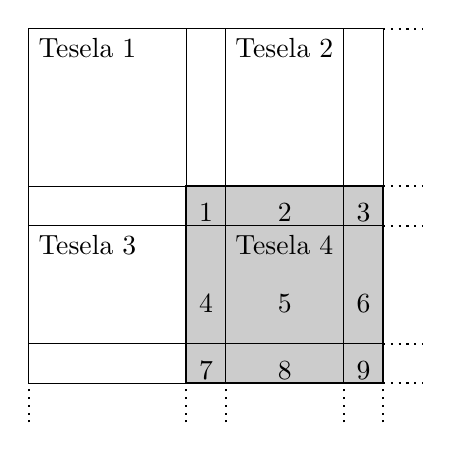
\begin{tikzpicture}[scale=0.50]
  \filldraw[fill=gray!40!white]   
    (4,0) -- (4,5) -- (9,5) -- (9,0) -- cycle;
  \draw (0,0) -- (0,5) -- (5,5) -- (5,0) -- cycle;
  \draw
    (0,4) node[anchor=north west] {Tesela 3} -- 
    (0,9) node[anchor=north west] {Tesela 1} -- 
    (5,9) node[anchor=north west] {Tesela 2} -- 
    (5,4) node[anchor=north west] {Tesela 4} -- cycle;
  \draw (4,4) -- (4,9) -- (9,9) -- (9,4) -- cycle;
  \draw
    (0,5) -- (4,5) -- node[below=.1cm] {1} 
    (5,5) -- node[below=0.1cm] {2} 
    (8,5) -- node[below=0.1cm] {3} (9,5); 
  \draw
    (0,1) -- (4,1) -- node[below=.1cm] {7} 
    (5,1) -- node[below=.1cm] {8} 
    (8,1) -- node[below=.1cm] {9} (9,1); 
  \draw
    (0,4) -- (4,4) -- node[below=.75cm] {4} 
    (5,4) -- node[below=.75cm] {5} 
    (8,4) -- node[below=.75cm] {6} (9,4); 
  \draw (4,0) -- (4,9); 
  \draw (8,0) -- (8,9); 
    % Continuacion de teselas en lineas de puntos
  \draw[thick] (4,0) -- (4,5) -- (9,5) -- (9,0) -- cycle;
  \draw[dotted,thick] (9,0) -- (10,0);
  \draw[dotted,thick] (9,1) -- (10,1);
  \draw[dotted,thick] (9,4) -- (10,4);
  \draw[dotted,thick] (9,5) -- (10,5);
  \draw[dotted,thick] (9,9) -- (10,9);
  \draw[dotted,thick] (0,-1) -- (0,0);
  \draw[dotted,thick] (4,-1) -- (4,0);
  \draw[dotted,thick] (5,-1) -- (5,0);
  \draw[dotted,thick] (8,-1) -- (8,0);
  \draw[dotted,thick] (9,-1) -- (9,0);
    \end{tikzpicture}
    \end{figure}
\end{frame}
%%==================================================================F
